%definira klasu dokumenta 
\documentclass[12pt]{report} 

%prostor izmedu naredbi \documentclass i \begin{document} se zove uvod. U njemu se nalaze naredbe koje se odnose na cijeli dokument

%osnovni LaTex ne može riješiti sve probleme, pa se koriste različiti paketi koji olakšavaju izradu željenog dokumenta
\usepackage[croatian]{babel} 
\usepackage{amssymb}
\usepackage{amsmath}
\usepackage{txfonts}
\usepackage{mathdots}
\usepackage{titlesec}
\usepackage{array}
\usepackage{lastpage}
\usepackage{etoolbox}
\usepackage{tabularray}
\usepackage{color, colortbl}
\usepackage{adjustbox}
\usepackage{geometry}
\usepackage[classicReIm]{kpfonts}
\usepackage{hyperref}
\usepackage{fancyhdr}

\usepackage{float}
\usepackage{setspace}
\restylefloat{table}


\patchcmd{\chapter}{\thispagestyle{plain}}{\thispagestyle{fancy}}{}{} %redefiniranje stila stranice u paketu fancyhdr

%oblik naslova poglavlja
\titleformat{\chapter}{\normalfont\huge\bfseries}{\thechapter.}{20pt}{\Huge}
\titlespacing{\chapter}{0pt}{0pt}{40pt}


\linespread{1.3} %razmak između redaka

\geometry{a4paper, left=1in, top=1in,}  %oblik stranice

\hypersetup{ colorlinks, citecolor=black, filecolor=black, linkcolor=black,	urlcolor=black }   %izgled poveznice


%prored smanjen između redaka u nabrajanjima i popisima
\newenvironment{packed_enum}{
	\begin{enumerate}
		\setlength{\itemsep}{0pt}
		\setlength{\parskip}{0pt}
		\setlength{\parsep}{0pt}
	}{\end{enumerate}}

\newenvironment{packed_item}{
	\begin{itemize}
		\setlength{\itemsep}{0pt}
		\setlength{\parskip}{0pt}
		\setlength{\parsep}{0pt}
	}{\end{itemize}}




%boja za privatni i udaljeni kljuc u tablicama
\definecolor{LightBlue}{rgb}{0.9,0.9,1}
\definecolor{LightGreen}{rgb}{0.9,1,0.9}

%Promjena teksta za dugačke tablice
\DefTblrTemplate{contfoot-text}{normal}{Nastavljeno na idućoj stranici}
\SetTblrTemplate{contfoot-text}{normal}
\DefTblrTemplate{conthead-text}{normal}{(Nastavljeno)}
\SetTblrTemplate{conthead-text}{normal}
\DefTblrTemplate{middlehead,lasthead}{normal}{Nastavljeno od prethodne stranice}
\SetTblrTemplate{middlehead,lasthead}{normal}

%podesavanje zaglavlja i podnožja

\pagestyle{fancy}
\lhead{Programsko inženjerstvo}
\rhead{ConnectiNET}
\lfoot{Kraljevi}
\cfoot{stranica \thepage/\pageref{LastPage}}
\rfoot{19. siječnja 2023.}
\renewcommand{\headrulewidth}{0.2pt}
\renewcommand{\footrulewidth}{0.2pt}


\begin{document} 
	
	
	
	\begin{titlepage}
		\begin{center}
			\vspace*{\stretch{1.0}} %u kombinaciji s ostalim \vspace naredbama definira razmak između redaka teksta
			\LARGE Programsko inženjerstvo\\
			\large Ak. god. 2023./2024.\\
			
			\vspace*{\stretch{3.0}}
			
			\huge ConnectiNET\\
			\Large Dokumentacija, Rev. \textit{2}\\
			
			\vspace*{\stretch{12.0}}
			\normalsize
			Grupa: \textit{Kraljevi}\\
			Voditelj: \textit{Luka Miličević}\\
			
			
			\vspace*{\stretch{1.0}}
			Datum predaje: \textit{19. 1. 2023.}\\
	
			\vspace*{\stretch{4.0}}
			
			Nastavnik: \textit{Doc. Dr. Sc. Nikolina Frid}\\
		
		\end{center}

	
	\end{titlepage}

	
	\tableofcontents


	\chapter{Dnevnik promjena dokumentacije}
		
		%\textbf{\textit{Kontinuirano osvježavanje}}\\		
		
		% Primjer:
		% \begin{longtblr}[
		% 		label=none
		% 	]{
		% 		width = \textwidth, 
		% 		colspec={|X[2]|X[13]|X[3]|X[3]|}, 
		% 		rowhead = 1
		% 	}
		% 	\hline
		% 	\textbf{Rev.}	& \textbf{Opis promjene/dodatka} & \textbf{Autori} & \textbf{Datum}\\[3pt] \hline
		% 	0.1 & Napravljen predložak.	& * & 22.08.2013. 		\\[3pt] \hline 
		% 	0.2	& Dopisane upute za povijest dokumentacije.\newline Dodane reference. & * & 24.08.2013. 	\\[3pt] \hline 
		% 	0.5 & Dodan \textit{Use Case} dijagram i jedan sekvencijski dijagram, funkcionalni i nefunkcionalni zahtjevi i dodatak A & * & 25.08.2013. \\[3pt] \hline 
		% 	0.6 & Arhitektura i dizajn sustava, algoritmi i strukture podataka & * & 26.08.2013. \\[3pt] \hline 
		% 	0.8 & Povijest rada i trenutni status implementacije,\newline Zaključci i plan daljnjeg rada & * & 28.08.2013. \\[3pt] \hline 
		% 	0.9 & Opisi obrazaca uporabe & * & 07.09.2013. \\[3pt] \hline 
		% 	0.10 & Preveden uvod & * & 08.09.2013. \\[3pt] \hline 
		% 	0.11 & Sekvencijski dijagrami & * & 09.09.2013. \\[3pt] \hline 
		% 	0.12.1 & Započeo dijagrame razreda & * & 10.09.2013. \\[3pt] \hline 
		% 	0.12.2 & Nastavak dijagrama razreda & * & 11.09.2013. \\[3pt] \hline 
		% 	\textbf{1.0} & Verzija samo s bitnim dijelovima za 1. ciklus & * & 11.09.2013. \\[3pt] \hline 
		% 	1.1 & Uređivanje teksta -- funkcionalni i nefunkcionalni zahtjevi & * \newline * & 14.09.2013. \\[3pt] \hline 
		% 	1.2 & Manje izmjene:Timer - Brojilo vremena & * & 15.09.2013. \\[3pt] \hline 
		% 	1.3 & Popravljeni dijagrami obrazaca uporabe & * & 15.09.2013. \\[3pt] \hline 
		% 	1.5 & Generalna revizija strukture dokumenta & * & 19.09.2013. \\[3pt] \hline 
		% 	1.5.1 & Manja revizija (dijagram razmještaja) & * & 20.09.2013. \\[3pt] \hline 
		% 	\textbf{2.0} & Konačni tekst predloška dokumentacije  & * & 28.09.2013. \\[3pt] \hline 
		% 	&  &  & \\[3pt] \hline	
		% \end{longtblr}

		\begin{longtblr}[
				label=none
			]{
				width = \textwidth, 
				colspec={|X[2]|X[13]|X[3]|X[3]|}, 
				rowhead = 1
			}
			\hline
			\textbf{Rev.}	& \textbf{Opis promjene/dodatka} & \textbf{Autori} & \textbf{Datum}\\[3pt] \hline
			0.1 & Uređena prva stranica, napravljen opis zadatka	& Luka Miličević & 31.10.2023.	\\[3pt] \hline 
			0.2 & Ostali zahtjevi, dnevnik promjena, dnevnik sastanaka, tablica aktivnosti - inicijalno postavljanje	& Luka Miličević & 31.10.2023.	\\[3pt] \hline 
			0.3 & Funkcionalni zahtjevi - dionici i aktori & Duje Huljev & 2.11.2023.	\\[3pt] \hline 
			0.4 & Obrasci uporabe 1-16	& Filip Aleksić, Erik Pužar & 2.11.2023.	\\[3pt] \hline 
			0.5 & Implementacija - korištene tehnologije u proteklom periodu razvoja & Domagoj Sviličić & 3.11.2023.	\\[3pt] \hline 
			0.6 & Entiteti baze podataka	& Stjepan Đelekovčan & 3.11.2023.	\\[3pt] \hline 
      		0.7 & Obrasci uporabe 17-25 & Mate Papak & 3.11.2023.	\\[3pt] \hline 
			0.8 & Arhitektura i dizajn sustava - opis i dijagrami razreda & Luka Miličević & 6.11.2023.	\\[3pt] \hline 
			0.9 & UC dijagrami & Filip ALeksić, Mate Papak, Duje Huljev, Erik Pužar & 6.11.2023.	\\[3pt] \hline 
			0.10 & Sekvencijski dijagram UC1 prva verzija & Domagoj Sviličić & 9.11.2023.	\\[3pt] \hline
			0.11 & Sekvencijski dijagram UC1 i UC12 & Domagoj Sviličić & 11.11.2023.	\\[3pt] \hline
			0.12 & Dorada relacijskog dijagrama	& Stjepan Đelekovčan & 12.11.2023.	\\[3pt] \hline 
			0.13 & Ispravak UC dijagrama & Duje Huljev & 12.11.2023.	\\[3pt] \hline  
			0.14 & Dorada dijagrama klasa - DTO i Controllers & Luka Miličević & 14.11.2023.	\\[3pt] \hline  
			\textbf{1.0} & Verzija samo s bitnim dijelovima za 1. ciklus & * & 17.11.2023. \\[3pt] \hline 
			1.1 & Implementacija & * & 10.1.2024. \\[3pt] \hline 
			1.2 & Dijagram aktivnosti & Domagoj Sviličić & 11.1.2024. \\[3pt] \hline 
			1.3 & Ažurirane tablice, opisi tablica, dijagram razreda i relacijski dijagram & Stjepan Đelekovčan & 15.1.2024. \\[3pt] \hline 
			1.4 & Korekcija informacija i dijagrama prema implementaciji & Luka Miličević & 16.1.2024. \\[3pt] \hline
			1.5 & Dijagram razmještaja, dijagram komponenti, korekcija dijagrama aktivnosti & Domagoj Sviličić & 17.1.2024. \\[3pt] \hline
			1.6 & Dopuna korištenih tehnologija & Domagoj Sviličić & 17.1.2024. \\[3pt] \hline  
			1.7 & Dijagram stanja & Duje Huljev & 17.1.2024. \\[3pt] \hline
			1.8 & Popravak detalja i dijagrama & Luka Miličević & 17.1.2024. \\[3pt] \hline
			1.9 & Dopuna korištenih tehnologija, ispravak svih use-case dijagrama, dijagrama razmještaja i UC5 sekvencijskog dijagrama, napravljen zaključak, dodana skica kod arhitekture & Domagoj Sviličić & 18.1.2024. \\[3pt] \hline   
			1.10 & Upute za puštanje u pogon & Luka Miličević & 18.1.2024. \\[3pt] \hline
			1.11 & Ispitivanje programske potpore, upis sati i konačna dorada & Luka Miličević, Mate Papak, Filip Aleksić & 19.1.2024. \\[3pt] \hline
			&  &  & \\[3pt] \hline	
		\end{longtblr}
	
	
		% \textit{Moraju postojati glavne revizije dokumenata 1.0 i 2.0 na kraju prvog i drugog ciklusa. Između tih revizija mogu postojati manje revizije već prema tome kako se dokument bude nadopunjavao. Očekuje se da nakon svake značajnije promjene (dodatka, izmjene, uklanjanja dijelova teksta i popratnih grafičkih sadržaja) dokumenta se to zabilježi kao revizija. Npr., revizije unutar prvog ciklusa će imati oznake 0.1, 0.2, …, 0.9, 0.10, 0.11.. sve do konačne revizije prvog ciklusa 1.0. U drugom ciklusu se nastavlja s revizijama 1.1, 1.2, itd.}
	\chapter{Opis projektnog zadatka}
		
		\textbf{\textit{dio 1. revizije}}\\
		
		\textit{Na osnovi projektnog zadatka detaljno opisati korisničke zahtjeve. Što jasnije opisati cilj projektnog zadatka, razraditi problematiku zadatka, dodati nove aspekte problema i potencijalnih rješenja. Očekuje se minimalno 3, a poželjno 4-5 stranica opisa.	Teme koje treba dodatno razraditi u ovom poglavlju su:}
		\begin{packed_item}
			\item \textit{potencijalna korist ovog projekta}
			\item \textit{postojeća slična rješenja (istražiti i ukratko opisati razlike u odnosu na zadani zadatak). Dodajte slike koja predočavaju slična rješenja.}
			\item \textit{skup korisnika koji bi mogao biti zainteresiran za ostvareno rješenje.}
			\item \textit{mogućnost prilagodbe rješenja }
			\item \textit{opseg projektnog zadatka}
			\item \textit{moguće nadogradnje projektnog zadatka}
		\end{packed_item}
		
		\textit{Za pomoć pogledati reference navedene u poglavlju „Popis literature“, a po potrebi konzultirati sadržaj na internetu koji nudi dobre smjernice u tom pogledu.}
		\eject
		
		\section{Primjeri u \LaTeX u}
		
		\textit{Ovo potpoglavlje izbrisati.}\\

		U nastavku se nalaze različiti primjeri kako koristiti osnovne funkcionalnosti \LaTeX a koje su potrebne za izradu dokumentacije. Za dodatnu pomoć obratiti se asistentu na projektu ili potražiti upute na sljedećim web sjedištima:
		\begin{itemize}
			\item Upute za izradu diplomskog rada u \LaTeX u - \url{https://www.fer.unizg.hr/_download/repository/LaTeX-upute.pdf}
			\item \LaTeX\ projekt - \url{https://www.latex-project.org/help/}
			\item StackExchange za Tex - \url{https://tex.stackexchange.com/}\\
		
		\end{itemize} 	


		
		\noindent \underbar{podcrtani tekst}, \textbf{podebljani tekst}, 	\textit{nagnuti tekst}\\
		\noindent \normalsize primjer \large primjer \Large primjer \LARGE {primjer} \huge {primjer} \Huge primjer \normalsize
				
		\begin{packed_item}
			
			\item  primjer
			\item  primjer
			\item  primjer
			\item[] \begin{packed_enum}
				\item primjer
				\item[] \begin{packed_enum}
					\item[1.a] primjer
					\item[b] primjer
				\end{packed_enum}
				\item primjer
			\end{packed_enum}
			
		\end{packed_item}
		
		\noindent primjer url-a: \url{https://www.fer.unizg.hr/predmet/proinz/projekt}
		
		\noindent posebni znakovi: \# \$ \% \& \{ \} \_ 
		$|$ $<$ $>$ 
		\^{} 
		\~{} 
		$\backslash$ 
		
		
		\begin{longtblr}[
			label=none,
			entry=none
			]{
				width = \textwidth,
				colspec={|X[8,l]|X[8, l]|X[16, l]|}, 
				rowhead = 1,
			} %definicija širine tablice, širine stupaca, poravnanje i broja redaka naslova tablice
			\hline \SetCell[c=3]{c}{\textbf{naslov unutar tablice}}	 \\ \hline[3pt]
			\SetCell{LightGreen}IDKorisnik & INT	&  	Lorem ipsum dolor sit amet, consectetur adipiscing elit, sed do eiusmod  	\\ \hline
			korisnickoIme	& VARCHAR &   	\\ \hline 
			email & VARCHAR &   \\ \hline 
			ime & VARCHAR	&  		\\ \hline 
			\SetCell{LightBlue} primjer	& VARCHAR &   	\\ \hline 
		\end{longtblr}
		

		\begin{longtblr}[
				caption = {Naslov s referencom izvan tablice},
				entry = {Short Caption},
			]{
				width = \textwidth, 
				colspec = {|X[8,l]|X[8,l]|X[16,l]|}, 
				rowhead = 1,
			}
			\hline
			\SetCell{LightGreen}IDKorisnik & INT	&  	Lorem ipsum dolor sit amet, consectetur adipiscing elit, sed do eiusmod  	\\ \hline
			korisnickoIme	& VARCHAR &   	\\ \hline 
			email & VARCHAR &   \\ \hline 
			ime & VARCHAR	&  		\\ \hline 
			\SetCell{LightBlue} primjer	& VARCHAR &   	\\ \hline 
		\end{longtblr}
	


		
		
		%unos slike
		\begin{figure}[H]
			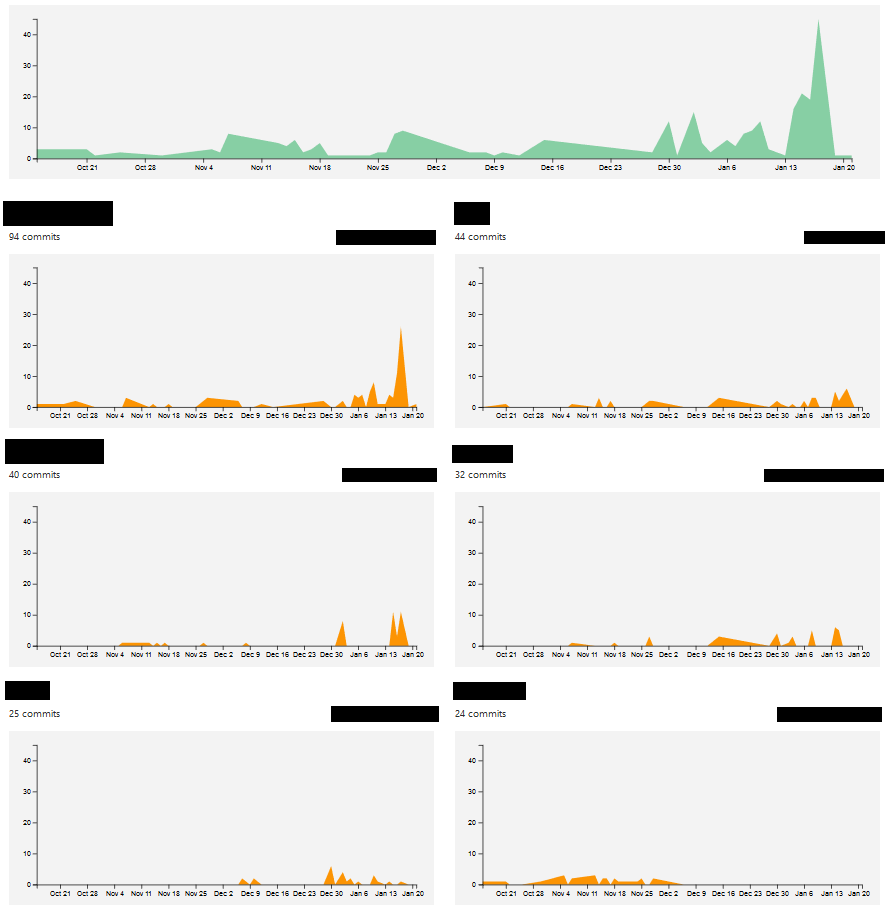
\includegraphics[scale=0.4]{slike/aktivnost.PNG} %veličina slike u odnosu na originalnu datoteku i pozicija slike
			\centering
			\caption{Primjer slike s potpisom}
			\label{fig:promjene}
		\end{figure}
		
		\begin{figure}[H]
			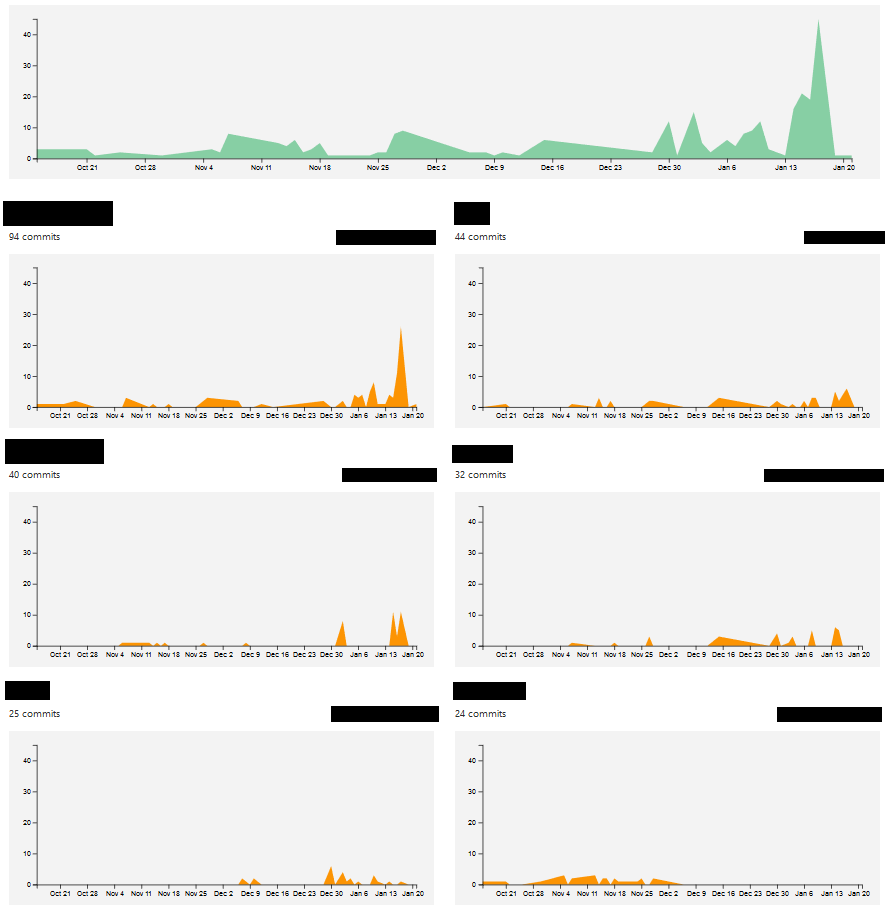
\includegraphics[width=\textwidth]{slike/aktivnost.PNG} %veličina u odnosu na širinu linije
			\caption{Primjer slike s potpisom 2}
			\label{fig:promjene2} %label mora biti drugaciji za svaku sliku
		\end{figure}
		
		Referenciranje slike \ref{fig:promjene2} u tekstu.
		
		\eject
		
	
	\chapter{Specifikacija programske potpore}
		
	\section{Funkcionalni zahtjevi}
			
			%\textbf{\textit{dio 1. revizije}}\\
			
			%\textit{Navesti \textbf{dionike} koji imaju \textbf{interes u ovom sustavu} ili  \textbf{su nositelji odgovornosti}. To su prije svega korisnici, ali i administratori sustava, naručitelji, razvojni tim.}\\
				
			%\textit{Navesti \textbf{aktore} koji izravno \textbf{koriste} ili \textbf{komuniciraju sa sustavom}. Oni mogu imati inicijatorsku ulogu, tj. započinju određene procese u sustavu ili samo sudioničku ulogu, tj. obavljaju određeni posao. Za svakog aktora navesti funkcionalne zahtjeve koji se na njega odnose.}\\
			
			
			\noindent \textbf{Dionici:}
			
			\begin{packed_enum}
				
				\item Vlasnik
				\item Klijenti
				\begin{packed_enum}
					\item Organizatori
					\item Posjetitelji
				\end{packed_enum}				
				\item Administratori
				\item Razvojni tim
				
			\end{packed_enum}
			
			\noindent \textbf{Aktori i njihovi funkcionalni zahtjevi:}

			\begin{packed_enum}
				\item \underbar{Neregistrirani/neprijavljeni korisnik (inicijator) može:}
				
				\begin{packed_enum}
					
					\item prijaviti se u sustav, unijeti korisničko ime i lozinku
					\item registrirati se u sustav, stvoriti korisnički račun za koji su mu potrebni korisničko ime, lozinka i e-mail adresa

				\end{packed_enum}

				\item \underbar{Prijavljeni korisnik (inicijator) može:}
				
				\begin{packed_enum}
					
					\item pregledati popis događaja
					\item kontrolirati način prikaza popisa događaja
					\begin{packed_enum}
						\item filtrirati događaje po kategoriji, lokaciji, vremenu održavanja
						\item sortirati događaje po kategoriji, udaljenosti, vremenu održavanja, cijeni, ocjeni
						\item pretraživati događaje po ključnim riječima
					\end{packed_enum}
					\item pregledati detalje događaja
					\item pregledati recenzije drugih posjetitelja
					\item odjaviti se iz sustava
					\item pregledati osobne podatke
					\item uređivati osobne podatke
					\item izbrisati svoj korisnički račun
					\item pregledati javni profil pojedinog organizatora
				\end{packed_enum}

				\item  \underbar{Organizator (inicijator) može:}
				
				\begin{packed_enum}
					
					\item sve što prijavljeni korisnik može
					\item stvoriti novi događaj i dodati mu potrebne informacije (opis, lokacija, vremenski raspored, cijena)
					\item uređivati vlastiti postojeći događaj
					\begin{packed_enum}
						
						\item izmijeniti nužne informacije o događaju (opis, lokacija, vremenski raspored, cijena)
						\item dodati, obrisati ili izmijeniti izborne informacije o događaju (slika, kategorija i sl.)
						
					\end{packed_enum}
					\item izbrisati vlastiti postojeći događaj
					\item pregledati statistiku za vlastite događaje
					\item dobiti uvid u recenzije događaja koje je organizirao
					\item odgovarati na recenzije na događaje koje je organizirao (extra?)
					\item uređivati ili skriti vlastiti javni profil
					\item upravljati pretplatom za premium organizatore
					\begin{packed_enum}
						
						\item pretplatiti se kao premium organizator putem PayPal-a ili kreditne kartice
						\item ukinuti pretplatu
						
					\end{packed_enum}
				
				\end{packed_enum}

				\item \underbar{Posjetitelj (inicijator) može:}
				
				\begin{packed_enum}
					
					\item sve što prijavljeni korisnik može
					\item odabrati i/ili promijeniti stupanj interesa za događaj („sigurno dolazim“, „možda dolazim“, „ne dolazim“)
					\item ostaviti i urediti recenziju za posjećeni događaj koji je završio unutar zadnjih 48h (ocjena, komentar)
					
				\end{packed_enum}
			
				\item  \underbar{Administrator (inicijator) može:}
				
				\begin{packed_enum}
					
					\item sve što prijavljeni korisnik može
					\item vidjeti popis svih registriranih korisnika i njihovih osobnih podataka
					\item dodavati nove administratore
					\item pristupiti statistici o korištenju aplikacije
					\item ukloniti recenzije koje krše pravila korištenja aplikacije
					\item ukloniti događaje koji krše pravila korištenja aplikacije
					\item ukloniti korisničke račune koji krše pravila korištenja aplikacije
					\item ukinuti pretplatu premium organizatorima koji krše pravila korištenja aplikacije
					\item postaviti cijenu članstva za premium organizatore					
				\end{packed_enum}

				\item  \underbar{Baza podataka (sudionik):}
				
				\begin{packed_enum}
					
					\item pohranjuje sve podatke o korisnicima, njihovim detaljima i ovlastima
					\item pohranjuje sve podatke o događajima, njihovim detaljima i recenzijama
					
				\end{packed_enum}
			\end{packed_enum}
			
			\eject 
			
			
				
			\subsection{Obrasci uporabe}
				
				%\textbf{\textit{dio 1. revizije}}
				
				\subsubsection{Opis obrazaca uporabe}
					%\textit{Funkcionalne zahtjeve razraditi u obliku obrazaca uporabe. Svaki obrazac je potrebno razraditi prema donjem predlošku. Ukoliko u nekom koraku može doći do odstupanja, potrebno je to odstupanje opisati i po mogućnosti ponuditi rješenje kojim bi se tijek obrasca vratio na osnovni tijek.}\\
					

					\noindent \underbar{\textbf{UC1 -Registracija}}
					\begin{packed_item}

						\item \textbf{Glavni sudionik:} Korisnik
						\item  \textbf{Cilj:} Stvoriti korisnicki račun za pristup sustavu
						\item  \textbf{Sudionici:} Baza podataka
						\item  \textbf{Preduvjet:} 
						\item  \textbf{Opis osnovnog tijeka:}

						\item[] \begin{packed_enum}

							\item Korisnik odabire opciju za registraciju
							\item Korisnik unosi potrebne korisničke podatke
							\item Korisnik prima obavijest o uspješnoj registraciji 

						\end{packed_enum}

						\item  \textbf{Opis mogućih odstupanja:}

						\item[] \begin{packed_item}

							\item[2.a] Odabir vec zauzetog korisničkog imena i/ili e-maila, unos korisničkog podatka u nedozvoljenom formatu ili pruzanje neispravnoga e-maila 
							\item[] \begin{packed_enum}

								\item Sustav obavjestava korisnika o neuspjelom upisu i vra ˇ ca ga na stra- ´
								nicu za registraciju
								\item Korisnik mijenja potrebne podatke te zavrsava unos ili odustaje od ˇ
								registracije

							\end{packed_enum}
						\end{packed_item}
					\end{packed_item}

					\noindent \underbar{\textbf{UC2 - Prijava}}
					\begin{packed_item}

						\item \textbf{Glavni sudionik:} Korisnik
						\item  \textbf{Cilj:} Dobiti pristup korisnickom sučelju
						\item  \textbf{Sudionici:} Baza podataka
						\item  \textbf{Preduvjet:} Registracija
						\item  \textbf{Opis osnovnog tijeka:}

						\item[] \begin{packed_enum}

							\item Unos korisničkog imena i lozinke
							\item Potvrda o ispravnosti unesenih podataka
							\item Pristup korisničkim funkcijama

						\end{packed_enum}

						\item  \textbf{Opis mogućih odstupanja:}

						\item[] \begin{packed_item}

							\item[2.a] Neispravno korisnicko ime/lozinka 
							\item[] \begin{packed_enum}

								\item Sustav obavjestava korisnika o neuspjelom upisu i vraća ga na stranicu za prijavu

							\end{packed_enum}

						\end{packed_item}
					\end{packed_item}


					\noindent \underbar{\textbf{UC3 - Pregled osobnih podataka}}
					\begin{packed_item}

						\item \textbf{Glavni sudionik:} Administrator, organizator, posjetitelj
						\item  \textbf{Cilj:} Pregledati osobne podatke
						\item  \textbf{Sudionici:} Baza podataka
						\item  \textbf{Preduvjet:} Korisnik je prijavljen
						\item  \textbf{Opis osnovnog tijeka:}

						\item[] \begin{packed_enum}

							\item Korisnik odabire opciju ”Osobni podatci”
							\item Aplikacija prikazuje osobne podatke korisnika

						\end{packed_enum}

					\end{packed_item}

					\noindent \underbar{\textbf{UC4 - Promjena osobnih podataka}}
					\begin{packed_item}

						\item \textbf{Glavni sudionik:} Organizator, posjetitelj
						\item  \textbf{Cilj:} Promijeniti osobne podatke
						\item  \textbf{Sudionici:} Baza podataka
						\item  \textbf{Preduvjet:} Organizator je prijavljen
						\item  \textbf{Opis osnovnog tijeka:}

						\item[] \begin{packed_enum}

							\item Korisnik odabere opciju za promjenu podataka
							\item Korisnik mijenja svoje osobne podatke
							\item Korisnik sprema promjene
							\item Baza podataka se ažurira

						\end{packed_enum}

						\item  \textbf{Opis mogućih odstupanja:}

						\item[] \begin{packed_item}

							\item[2.a] Korisnik promijeni svoje osobne podatke, ali ne odabere opciju ”Spremi
							promjenu”
							\item[] \begin{packed_enum}

								\item Sustav obavjestava korisnika da nije spremio podatke prije izlaska ˇ
								iz prozora

							\end{packed_enum}

						\end{packed_item}

					\end{packed_item}

					\noindent \underbar{\textbf{UC5 - Brisanje računa}}
					\begin{packed_item}

						\item \textbf{Glavni sudionik:} Administrator, korisnik
						\item  \textbf{Cilj:} Izbrisati svoj korisnički račun
						\item  \textbf{Sudionici:} Baza podataka
						\item  \textbf{Preduvjet:} Korisnik je prijavljen
						\item  \textbf{Opis osnovnog tijeka:}

						\item[] \begin{packed_enum}

							\item Korisnik pregledava osobne podatke
							\item Otvara se stranica s osobnim podacima korisnika
							\item Korisnik brise račun
							\item Korisnicki račun se izbriše iz baze podataka
							\item Otvara se stranica za registraciju
						\end{packed_enum}

						\item  \textbf{Opis mogućih odstupanja:}


					\end{packed_item}

					\noindent \underbar{\textbf{UC6 - Pregled popisa događaja}}
					\begin{packed_item}

						\item \textbf{Glavni sudionik:} Administrator, korisnik
						\item  \textbf{Cilj:} Pregledati nadolazeće događaje
						\item  \textbf{Sudionici:} Baza podataka
						\item  \textbf{Preduvjet:} Korisnik je prijavljen
						\item  \textbf{Opis osnovnog tijeka:}

						\item[] \begin{packed_enum}

							\item Korisniku se prikazuje popis aktualnih događaja 

						\end{packed_enum}

					\end{packed_item}

					\noindent \underbar{\textbf{UC7 - Kontrola pregleda popisa događaja}}
					\begin{packed_item}

						\item \textbf{Glavni sudionik:} Administrator, korisnik
						\item  \textbf{Cilj:} Prikaz događaja po korisnikovoj želji
						\item  \textbf{Sudionici:} Baza podataka
						\item  \textbf{Preduvjet:} Korisnik je prijavljen
						\item  \textbf{Opis osnovnog tijeka:}

						\item[] \begin{packed_enum}

							\item Korisnik ima mogućost filtriranja događaja po kategorijama, lokacijama te vremenu izvođenja događaja
							\item Korisnik ima mogućnost sortiranja događaja po kategorijama, lokacijama te vremenu izvođenja događaja
							\item Korisnik ima mogućnost traženja neke ključne riječi

						\end{packed_enum}


					\end{packed_item}

					\noindent \underbar{\textbf{UC8 - Pregled podataka o događaju}}
					\begin{packed_item}

						\item \textbf{Glavni sudionik:} Administrator, korisnik
						\item  \textbf{Cilj:} Prikaz detalja o odabranom događaju
						\item  \textbf{Sudionici:} Baza podataka
						\item  \textbf{Preduvjet:} Korisnik je prijavljen
						\item  \textbf{Opis osnovnog tijeka:}

						\item[] \begin{packed_enum}

							\item Korisnik odabire događaj
							\item Prikazuje mu se detalji o događaju poput naziva, vrste, lokacije, vremena početka, trajanja, foto/video galerije te popis recenzija

						\end{packed_enum}


					\end{packed_item}

					\noindent \underbar{\textbf{UC9 - Odabir stupnja interesa za događaj}}
					\begin{packed_item}
	
						\item \textbf{Glavni sudionik:} Posjetitelj
						\item  \textbf{Cilj:} Odabir interesa
						\item  \textbf{Sudionici:} Baza podataka
						\item  \textbf{Preduvjet:} Posjetitelj je prijavljen
						\item  \textbf{Opis osnovnog tijeka:}
						
						\item[] \begin{packed_enum}
	
							\item Posjetitelj otvara stranicu s popisom događaja
							\item Odabire događaj
							\item Odabire stupanj interesa između „sigurno dolazim“, „možda dolazim“ i „ne dolazim“

						\end{packed_enum}
					\end{packed_item}

					\noindent \underbar{\textbf{UC10 - Ostavljanje recenzije na dogadaj}}
					\begin{packed_item}
	
						\item \textbf{Glavni sudionik:} Posjetitelj
						\item  \textbf{Cilj:} Ostaviti recenziju
						\item  \textbf{Sudionici:} Baza podataka
						\item  \textbf{Preduvjet:} Posjetitelj je prijavljen i nije prošlo 48h od završetka događaja

						\item  \textbf{Opis osnovnog tijeka:}
						
						\item[] \begin{packed_enum}
	
							\item Posjetitelj otvara stranicu s popisom događaja
							\item Odabire događaj
							\item Posjetitelj odabire opciju "Ostavi recenziju"
							\item Posjetitelj piše recenziju
							\item Posjetitelj odabire opciju "Potvrdi recenziju"
							
						\end{packed_enum}
						
						\item  \textbf{Opis mogućih odstupanja:}
						
						\item[] \begin{packed_item}
	
							\item[5.a] Korisnik nije ispravno popunio obrazac za recenziju
							\begin{packed_enum}
								\item Sustav prikazuje poruku "Neispravno popunjen obrazac"
							\end{packed_enum}
							
						\end{packed_item}
					\end{packed_item}

					\noindent \underbar{\textbf{UC11 - Uvid u recenzije drugih posjetitelja}}
					\begin{packed_item}
	
						\item \textbf{Glavni sudionik:} Organizator, posjetitelj
						\item  \textbf{Cilj:} Pregledati recenzije
						\item  \textbf{Sudionici:} Baza podataka
						\item  \textbf{Preduvjet:} Organizator/posjetitelj je prijavljen
						\item  \textbf{Opis osnovnog tijeka:}
						
						\item[] \begin{packed_enum}
	
							\item Posjetitelj otvara stranicu s popisom događaja
							\item Odabire događaj
							\item Posjetitelj odabire opciju "Prikaži recenzije"

						\end{packed_enum}
						
						\item  \textbf{Opis mogućih odstupanja:}
						
						\item[] \begin{packed_item}
	
							\item[3.a] Događaj nema ni jednu recenziju
							\begin{packed_enum}
								\item Sustav prikazuje poruku "Nema recenzija za ovaj događaj"
							\end{packed_enum}
							
						\end{packed_item}
					\end{packed_item}

					\noindent \underbar{\textbf{UC12 - Organizacija vlastitog događaja}}
					\begin{packed_item}
	
						\item \textbf{Glavni sudionik:} Organizator
						\item  \textbf{Cilj:} Organizacija događaja
						\item  \textbf{Sudionici:} Baza podataka
						\item  \textbf{Preduvjet:} Organizator je prijavljen i ima premium verziju
						\item  \textbf{Opis osnovnog tijeka:}
						
						\item[] \begin{packed_enum}
	
							\item Organizator odabire opciju "Kreiraj novi događaj"
							\item Organizator upisuje detalje o događaju
							\item Organizator odabire opciju "Kreiraj događaj"

						\end{packed_enum}
						
						\item  \textbf{Opis mogućih odstupanja:}
						
						\item[] \begin{packed_item}
	
							\item[4.a] nisu popunjena nužna polja za stvaranje događaja
							\item[] \begin{packed_enum}
								
								\item Sustav prikazuje poruku "Neispravno popunjen obrazac"
								
							\end{packed_enum}
							
						\end{packed_item}
					\end{packed_item}

					\noindent \underbar{\textbf{UC13 - Uređivanje vlastitog dogadaja}}
					\begin{packed_item}
	
						\item \textbf{Glavni sudionik:} Organizator
						\item  \textbf{Cilj:} Uređivanje događaja
						\item  \textbf{Sudionici:} Baza podataka
						\item  \textbf{Preduvjet:} Organizator je prijavljen i ima kreirani događaj

						\item  \textbf{Opis osnovnog tijeka:}
						
						\item[] \begin{packed_enum}
	
							\item Organizator odabire opciju "Moji događaji"
							\item Organizator odabire događaj
							\item Organizator odabire opciju "Uredi događaj"
							\item Organizator uređuje detalje o događaju
							\item Organizator odabire opciju "Pohrani promjene"
						\end{packed_enum}

						\item[] \begin{packed_item}
	
							\item[4.a] nisu popunjena nužna polja za stvaranje događaja
							\item[] \begin{packed_enum}
								
								\item Sustav prikazuje poruku "Neispravno popunjen obrazac"
								
							\end{packed_enum}
							
						\end{packed_item}
						
					\end{packed_item}

					\noindent \underbar{\textbf{UC14 - Pregled podataka o vlastitom događaju}}
					\begin{packed_item}
	
						\item \textbf{Glavni sudionik:} Organizator
						\item  \textbf{Cilj:} Pregled podataka o kreiranom događaju
						\item  \textbf{Sudionici:} Baza podataka
						\item  \textbf{Preduvjet:} Organizator je prijavljen i ima kreirani događaj
						\item  \textbf{Opis osnovnog tijeka:}
						
						\item[] \begin{packed_enum}
	
							\item Organizator otvara stranicu s popisom događaja
							\item Organizator odabire opciju "Moji događaji"
							\item Organizator odabire događaj

						\end{packed_enum}
						
						\item  \textbf{Opis mogućih odstupanja:}
						
						\item[] \begin{packed_item}
	
							\item[2.a] Ne postoji niti jedan kreirani događaj
							\item[] \begin{packed_enum}
								
								\item Sustav prikazuje poruku "Nema događaja za prikazati"
								
							\end{packed_enum}
							
						\end{packed_item}
					\end{packed_item}

					\noindent \underbar{\textbf{UC15 - Pregled profila organizatora}}
					\begin{packed_item}
	
						\item \textbf{Glavni sudionik:} Administrator, korisnik
						\item  \textbf{Cilj:} Pregled podataka o organizatoru događaja
						\item  \textbf{Sudionici:} Baza podataka
						\item  \textbf{Preduvjet:} Korisnik je prijavljen
						\item  \textbf{Opis osnovnog tijeka:}
						
						\item[] \begin{packed_enum}
	
							\item Posjetitelj otvara stranicu s popisom događaja
							\item Posjetitelj odabire događaj
							\item Posjetitelj odabire opciju "Posjeti profil organizatora događaja"

						\end{packed_enum}

					\end{packed_item}

					\noindent \underbar{\textbf{UC16 - Pretplata}}
					\begin{packed_item}
	
						\item \textbf{Glavni sudionik:} Organizator
						\item  \textbf{Cilj:} Pretplacivanje
						\item  \textbf{Sudionici:} Baza podataka
						\item  \textbf{Preduvjet:} Organizator je prijavljen i nije pretplaćen
						\item  \textbf{Opis osnovnog tijeka:}
						
						\item[] \begin{packed_enum}
	
							\item Organizator odabire opciju "Osobni podatci"
							\item Organizator odabire opciju "Pretplata"
							\item Organizator odabire opciju "Pretplati se na ConnectiNET Premium"
							\item Organizator odabire vrstu plaćanja
							\item Organizator upisuje podatke potrebne za plaćanje
							\item Organizator odabire opciju "Potvrdi pretplatu"

						\end{packed_enum}
						
						\item  \textbf{Opis mogućih odstupanja:}
						
						\item[] \begin{packed_item}
	
							\item[5.a] Uneseni su neispravni bankovni podatci
							\item[] \begin{packed_enum}
								
								\item Sustav prikazuje poruku "Neispravni podaci o plaćanju"
								
							\end{packed_enum}
							\item[6.a] Stanje na bankovnom računu je manje od iznosa pretplate
							
						\end{packed_item}
					\end{packed_item}

					\noindent \underbar{\textbf{UC17 - Otkazivanje pretplate}}
					\begin{packed_item}
	
						\item \textbf{Glavni sudionik:} Organizator
						\item  \textbf{Cilj:} Otkazivanje pretplate
						\item  \textbf{Sudionici:} Baza podataka
						\item  \textbf{Preduvjet:} Organizator je prijavljen i ima pretplatu
						\item  \textbf{Opis osnovnog tijeka:}
						
						\item[] \begin{packed_enum}
	
							\item Organizator odabire opciju "Osobni podatci"
							\item Organizator odabire opciju "Pretplate"
							\item Organizator odabire opciju "Otkaži Premium pretplatu"
							\item Organizator odabire opciju "Da, otkaži pretplatu"
							\item Pretplata je otkazana
						\end{packed_enum}
						
						\item  \textbf{Opis mogućih odstupanja:}
						
						\item[] \begin{packed_item}
	
							\item[4.a] Organizator ipak ne želi otkazati pretplatu
							\item[] \begin{packed_enum}
								
								\item Organizator odabire opciju "Poništi"
								
							\end{packed_enum}
						\end{packed_item}
					\end{packed_item}
					
					\noindent \underbar{\textbf{UC18 - Primanje obavijesti o događajima}}
					\begin{packed_item}
	
						\item \textbf{Glavni sudionik:} Posjetitelj
						\item  \textbf{Cilj:} Primanje obavijesti o događajima
						\item  \textbf{Sudionici:} Baza podataka
						\item  \textbf{Preduvjet:} Posjetitelj je prijavljen i ***
						\item  \textbf{Opis osnovnog tijeka:}
						
						\item[] \begin{packed_enum}
	
							\item ***Ovdje se moramo kao grupa dogovoriti koliko komplicirat želimo
						\end{packed_enum}
					\end{packed_item}

					\noindent \underbar{\textbf{UC19 - Postavljanje cijene pretplate}}
					\begin{packed_item}
	
						\item \textbf{Glavni sudionik:} Administrator
						\item  \textbf{Cilj:} Postavljanje cijene pretplate
						\item  \textbf{Sudionici:} Baza podataka
						\item  \textbf{Preduvjet:} Administrator je prijavljen
						\item  \textbf{Opis osnovnog tijeka:}
						
						\item[] \begin{packed_enum}
	
							\item Administrator odabire opciju "Administratorske postavke"
							\item Administrator odabire opciju "Premium pretplate"
							\item Administrator upisuje željenu cijenu (u eurima) na mjesto "Cijena:"
						\end{packed_enum}
					\end{packed_item}

					\noindent \underbar{\textbf{UC20 - Uklanjanje korisnika}}
					\begin{packed_item}
	
						\item \textbf{Glavni sudionik:} Administrator
						\item  \textbf{Cilj:} Uklanjanje korisnika
						\item  \textbf{Sudionici:} Baza podataka
						\item  \textbf{Preduvjet:} Administrator je prijavljen i korisnik postoji
						\item  \textbf{Opis osnovnog tijeka:}
						
						\item[] \begin{packed_enum}
	
							\item Administrator odabire opciju "Administratorske postavke"
							\item Administrator odabire opciju "Korisnici"
							\item Administrator upisuje ime korisnika u tražilicu
							\item Svi korisnici s navedenim pretraživanjem u imenu se prikazuju
							\item Administrator odabire željenog korisnika
							\item Administrator odabire opciju "Ukloni korisnika"
							\item Administrator odabire opciju "Da, ukloni korisnika"
							\item Korisnik je uklonjen
						\end{packed_enum}
						
						\item  \textbf{Opis mogućih odstupanja:}
						
						\item[] \begin{packed_item}
						
							\item[3.a] Administrator odabire filter "Organizator" ili "Posjetitelj" umjesto "Svi"
							\item[3.b] Administrator odabire vrstu sortiranja rezultata
							\item[4.a] Korisnik ne postoji
							\item[7.a] Administrator ipak ne želi ukloniti korisnika
							\item[] \begin{packed_enum}
								
								\item Administrator odabire opciju "Poništi"
								
							\end{packed_enum}
						\end{packed_item}
					\end{packed_item}

					\noindent \underbar{\textbf{UC21 - Uklanjanje recenzija}}
					\begin{packed_item}
	
						\item \textbf{Glavni sudionik:} Administrator
						\item  \textbf{Cilj:} Uklanjanje recenzija
						\item  \textbf{Sudionici:} Baza podataka
						\item  \textbf{Preduvjet:} Administrator je prijavljen i recenzija postoji
						\item  \textbf{Opis osnovnog tijeka:}
						
						\item[] \begin{packed_enum}
	
							\item Administrator odabire opciju "Administratorske postavke"
							\item Administrator odabire opciju "Korisnici"
							\item Administrator upisuje ime korisnika u tražilicu
							\item Svi korisnici s navedenim pretraživanjem u imenu se prikazuju
							\item Administrator odabire željenog korisnika
							\item Administrator odabire opciju "Recenzije"
							\item Administrator upisuje ime događaja u tražilicu
							\item Administrator odabire željeni događaj
							\item Korisnikova recenzija odabranog događaja se prikazuje
							\item Administrator odabire opciju "Ukloni recenziju"
							\item Administrator odabire opciju "Da, ukloni recenziju"
							\item Recenzija je uklonjena
						\end{packed_enum}
						
						\item  \textbf{Opis mogućih odstupanja:}
						
						\item[] \begin{packed_item}
	
							\item[3.a] Administrator odabire filter "Organizator" ili "Posjetitelj" umjesto "Svi"
							\item[3.b] Administrator odabire vrstu sortiranja rezultata
							\item[4.a] Korisnik ne postoji
							\item[11.a] Administrator ipak ne želi ukloniti korisnika
							\item[] \begin{packed_enum}
								
								\item Administrator odabire opciju "Poništi"
								
							\end{packed_enum}
						\end{packed_item}
					\end{packed_item}

					\noindent \underbar{\textbf{UC22 - Uklanjanje pretplate}}
					\begin{packed_item}
	
						\item \textbf{Glavni sudionik:} Administrator
						\item  \textbf{Cilj:} Uklanjanje pretplate
						\item  \textbf{Sudionici:} Baza podataka
						\item  \textbf{Preduvjet:} Administrator je prijavljen i organizacija postoji
						\item  \textbf{Opis osnovnog tijeka:}
						
						\item[] \begin{packed_enum}
	
							\item Administrator odabire opciju "Administratorske postavke"
							\item Administrator odabire opciju "Korisnici"
							\item Administrator odabire filter "Organizator" (preporučeno)
							\item Administrator upisuje ime organizatora u tražilicu
							\item Svi organizatori s navedenim pretraživanjem u imenu se prikazuju
							\item Administrator odabire željenog organizatora
							\item Administrator odabire opciju "Pretplata"
							\item Administrator odabire opciju "Ukloni Premium pretplatu"
							\item Administrator odabire opciju "Da, ukloni pretplatu"
							\item Pretplata je uklonjena
						\end{packed_enum}
						
						\item  \textbf{Opis mogućih odstupanja:}
						
						\item[] \begin{packed_item}
	
							\item[3.b] Administrator odabire vrstu sortiranja rezultata
							\item[5.a] Organizator ne postoji
							\item[8.a] Organizator već nema Premium pretplatu
							\item[9.a] Administrator ipak ne želi ukloniti pretplatu
							\item[] \begin{packed_enum}
								
								\item Administrator odabire opciju "Poništi"
								
							\end{packed_enum}
						\end{packed_item}
					\end{packed_item}

					\noindent \underbar{\textbf{UC23 - Uklanjanje događaja}}
					\begin{packed_item}
	
						\item \textbf{Glavni sudionik:} Administrator
						\item  \textbf{Cilj:} Uklanjanje događaja
						\item  \textbf{Sudionici:} Baza podataka
						\item  \textbf{Preduvjet:} Administrator je prijavljen i događaj postoji
						\item  \textbf{Opis osnovnog tijeka:}
						
						\item[] \begin{packed_enum}
	
							\item Administrator odabire opciju "Administratorske postavke"
							\item Administrator odabire opciju "Korisnici"
							\item Administrator odabire filter "Organizator" (preporučeno)
							\item Administrator upisuje ime organizatora u tražilicu
							\item Svi organizatori s navedenim pretraživanjem u imenu se prikazuju
							\item Administrator odabire željenog organizatora
							\item Administrator odabire opciju "Događaji"
							\item Administrator upisuje ime događaja u tražilicu
							\item Korisnikova recenzija odabranog događaja se prikazuje
							\item Administrator odabire opciju "Ukloni događaj"
							\item Administrator odabire opciju "Da, ukloni događaj"
							\item Događaj je uklonjen
						\end{packed_enum}
						
						\item  \textbf{Opis mogućih odstupanja:}
						
						\item[] \begin{packed_item}
	
							\item[3.b] Administrator odabire vrstu sortiranja rezultata
							\item[5.a] Organizator ne postoji
							\item[9.a] Administrator ipak ne želi ukloniti pretplatu
							\item[] \begin{packed_enum}
								
								\item Administrator odabire opciju "Poništi"
								
							\end{packed_enum}
						\end{packed_item}
					\end{packed_item}
				
					\noindent \underbar{\textbf{UC24 - Dodavanje administratora}}
					\begin{packed_item}
	
						\item \textbf{Glavni sudionik:} Administrator
						\item  \textbf{Cilj:} Dodavanje administratora
						\item  \textbf{Sudionici:} Baza podataka
						\item  \textbf{Preduvjet:} Administrator je prijavljen
						\item  \textbf{Opis osnovnog tijeka:}
						
						\item[] \begin{packed_enum}
	
							\item Administrator odabire opciju "Administratorske postavke"
							\item Administrator odabire opciju "Administratori"
							\item Administrator odabire opciju "Dodaj novog administratora"
							\item Administrator upisuje email novog administratora
							\item Administrator odabire opciju "Dodaj administratora"
							\item Administrator odabire opciju "Da, dodaj administratora"
							\item Administrator je dodan
						\end{packed_enum}
						
						\item  \textbf{Opis mogućih odstupanja:}
						
						\item[] \begin{packed_item}
	
							\item[6.a] Administrator ipak ne želi dodati administratora
							\item[] \begin{packed_enum}
								
								\item Administrator odabire opciju "Poništi"
								
							\end{packed_enum}
						\end{packed_item}
					\end{packed_item}

					\noindent \underbar{\textbf{UC25 - Pregled statistike}}
					\begin{packed_item}
	
						\item \textbf{Glavni sudionik:} Administrator
						\item  \textbf{Cilj:} Pregled statistike
						\item  \textbf{Sudionici:} Baza podataka
						\item  \textbf{Preduvjet:} Administrator je prijavljen
						\item  \textbf{Opis osnovnog tijeka:}
						
						\item[] \begin{packed_enum}
	
							\item Administrator odabire opciju "Administratorske postavke"
							\item Administrator odabire opciju "Statistika"
							\item Administratoru se prikažu različite statistike vezane za pretplate, događaje i korisnike
						\end{packed_enum}
					\end{packed_item}

					\noindent \underbar{\textbf{UC26 - Uređivanje javnog profila}}
					\begin{packed_item}
	
						\item \textbf{Glavni sudionik:} Organizator
						\item  \textbf{Cilj:} Uređivanje javnog profila
						\item  \textbf{Sudionici:} Baza podataka
						\item  \textbf{Preduvjet:} Organizator ima kreiran javni profil
						\item  \textbf{Opis osnovnog tijeka:}
						
						\item[] \begin{packed_enum}
	
							\item Organizator odabire opciju "Osobni podatci"
							\item Organizator odabire opciju "Javni profil"
							\item Organizator odabire opciju "Uredi javni profil"
							\item Organizator unosi podatke o sebi
							\item Organizator odabire opciju "Potvrdi promjene"
						\end{packed_enum}

						\item  \textbf{Opis mogućih odstupanja:}
						
						\item[] \begin{packed_item}
	
							\item[5.a] Organizator je napravio neispravne promjene
							\item[] \begin{packed_enum}
								
								\item Sustav prikazuje poruku "Neispravno popunjen obrazac"
								
							\end{packed_enum}
						\end{packed_item}
					\end{packed_item}

					\noindent \underbar{\textbf{UC27 - Skrivanje javnog profila}}
					\begin{packed_item}
	
						\item \textbf{Glavni sudionik:} Organizator
						\item  \textbf{Cilj:} Skrivanje javnog profila
						\item  \textbf{Sudionici:} Baza podataka
						\item  \textbf{Preduvjet:} Organizator ima kreiran javni profil
						\item  \textbf{Opis osnovnog tijeka:}
						
						\item[] \begin{packed_enum}
	
							\item Organizator odabire opciju "Osobni podatci"
							\item Organizator odabire opciju "Javni profil"
							\item Organizator odabire opciju "Sakrij javni profil"
							\item Organizator odabire opciju "Potvrdi"
						\end{packed_enum}

						\item  \textbf{Opis mogućih odstupanja:}
						
						\item[] \begin{packed_item}
	
							\item[4.a] Organizator ipak ne želi izbrisati skriti profil
							\item[] \begin{packed_enum}
								
								\item Organizator odabire opciju "Poništi"
								
							\end{packed_enum}
						\end{packed_item}
					\end{packed_item}
					
				\subsubsection{Dijagrami obrazaca uporabe}
					
					%\textit{Prikazati odnos aktora i obrazaca uporabe odgovarajućim UML dijagramom. Nije nužno nacrtati sve na jednom dijagramu. Modelirati po razinama apstrakcije i skupovima srodnih funkcionalnosti.}

					\begin{figure}[htbp]
						\centering
						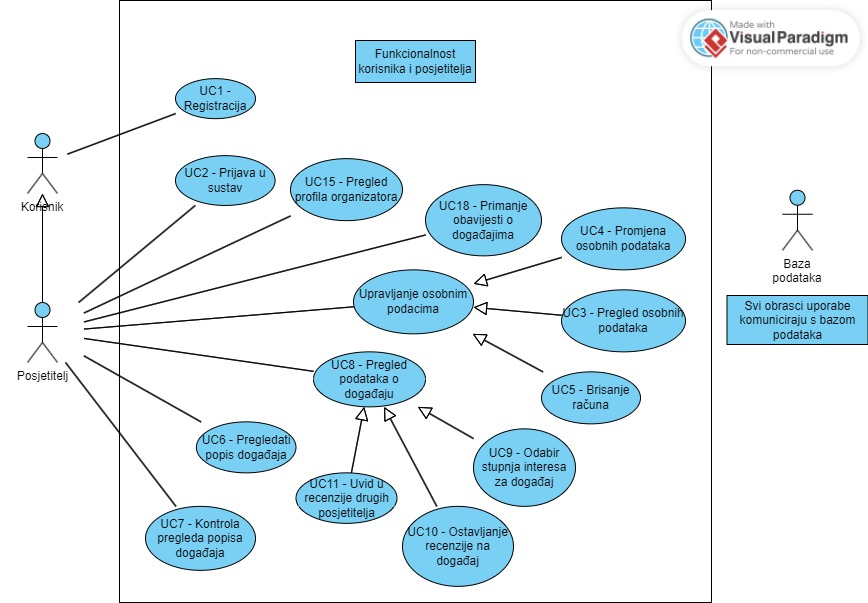
\includegraphics[width=1\textwidth]{dijagrami/obrazac_funkcionalnost_posjetitelja.jpg}
						\caption{Dijagram obrasca uporabe, funkcionalnost posjetitelja}
					\label{fig:my_image}
					\end{figure}
					
					\begin{figure}[htbp]
						\centering
						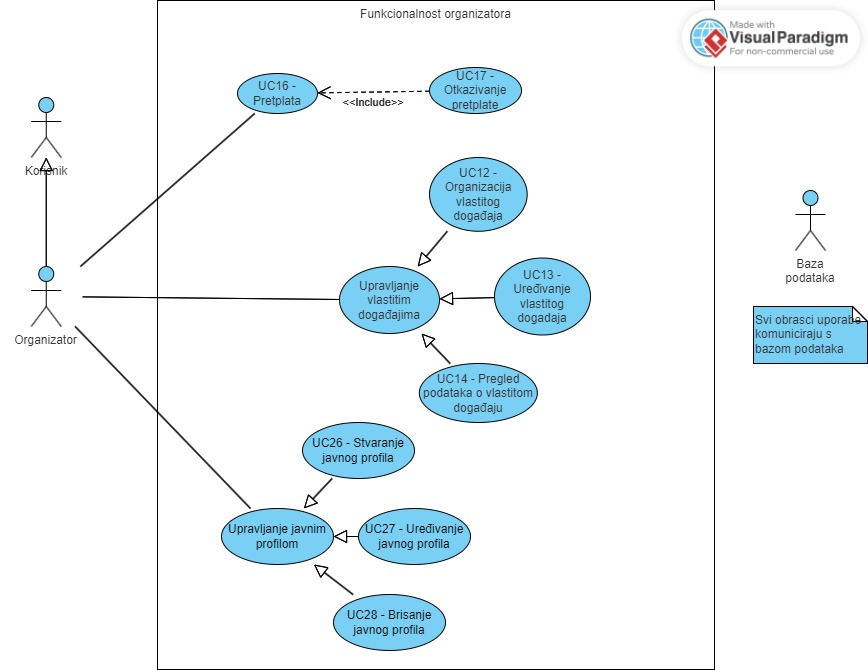
\includegraphics[width=1\textwidth]{dijagrami/obrazac_funkcionalnost_organizatora.jpg}
						\caption{Dijagram obrasca uporabe, funkcionalnost organizatora}
					\label{fig:my_image}
					\end{figure}

					\begin{figure}[htbp]
						\centering
						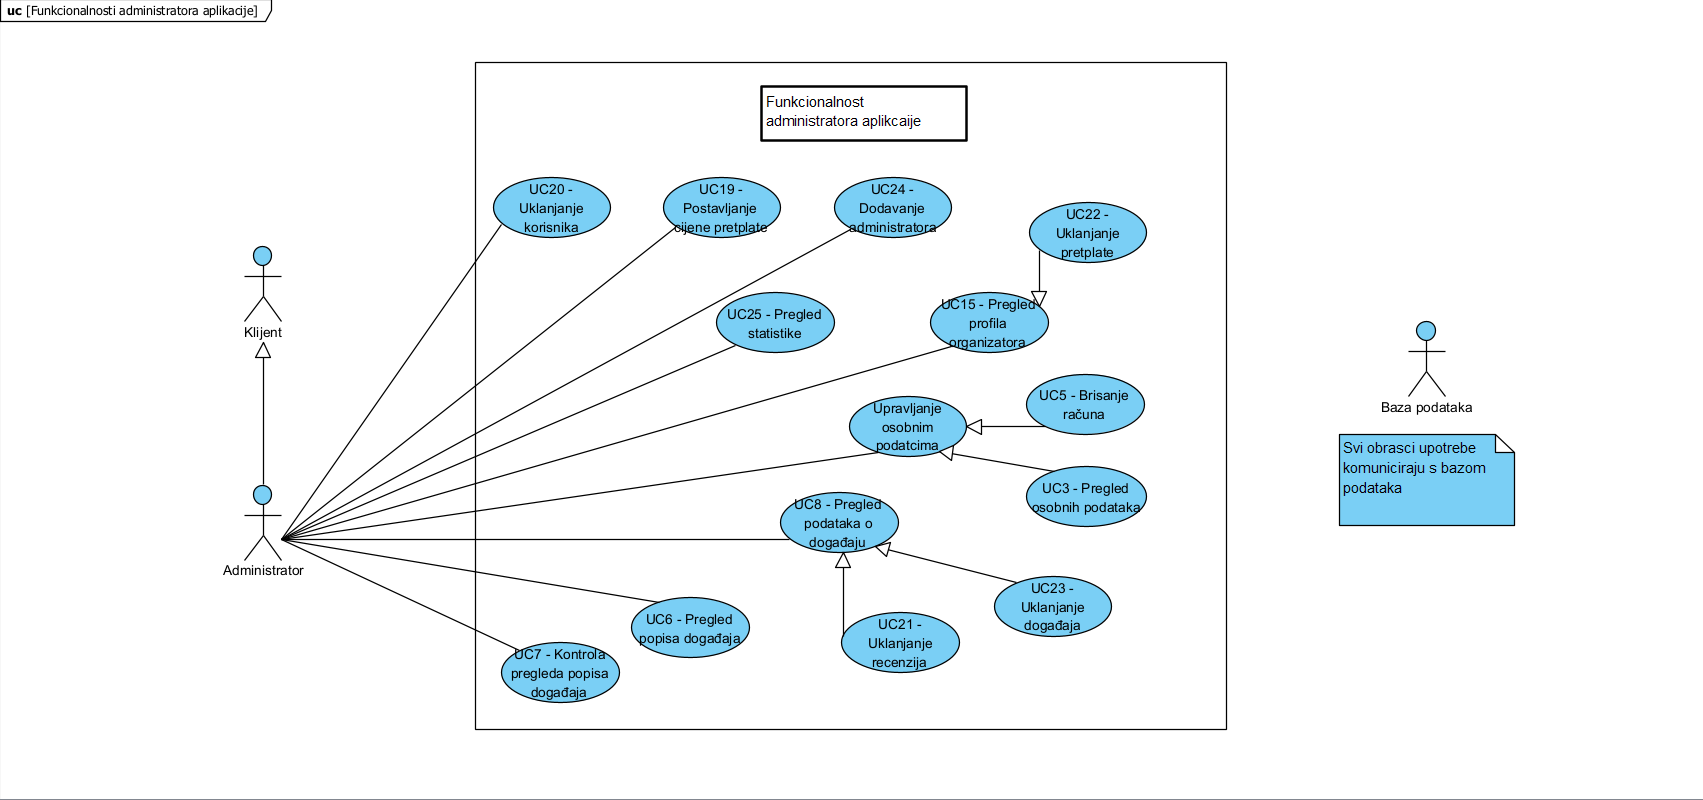
\includegraphics[width=1\textwidth]{dijagrami/obrazac_funkcionalnost_administratora.png}
						\caption{Dijagram obrasca uporabe, funkcionalnost administratora}
					\label{fig:my_image}
					\end{figure}

				\eject		
				
			\subsection{Sekvencijski dijagrami}
				
				%\textbf{\textit{dio 1. revizije}}\\
				
				%\textit{Nacrtati sekvencijske dijagrame koji modeliraju najvažnije dijelove sustava (max. 4 dijagrama). Ukoliko postoji nedoumica oko odabira, razjasniti s asistentom. Uz svaki dijagram napisati detaljni opis dijagrama.}

				\noindent \textbf{UC10 - Ostavljanje recenzije na dogadaj}

				\noindent Posjetitelj šalje zahtjev za prikaz događaja na kojima je bio 
				(kartica "Moji događaji") kako bi mogao odabrati događaj na kojem
				želi ostaviti recenziju. Poslužitelj dohvaća takve događaje iz baze podataka
				i prikazuje ih. Odabirom događaja, poslužitelj dohvaća podatke o događaju
				i prikazuje ih posjetitelju. Posjetitelj odabire opciju "Ostavi recenziju"
				te mu se prikazuje obrazac za ostavljanje recenzije. Posjetitelj unosi
				ocjenu i komentar te odabire opciju "Potvrdi recenziju". Poslužitelj
				sprema recenziju u bazu podataka i prikazuje poruku o uspješnom ostavljanju
				recenzije. Ako posjetitelj nije odabrao ocjenu ili nije unio komentar,
				prikazuje se poruka o neispravno popunjenom obrascu. Ako se posjetitelj
				predomisli, može odabrati opciju "Poništi" te se vraća na stranicu s
				podacima o događaju.

				\begin{figure}[htbp]
					\centering
					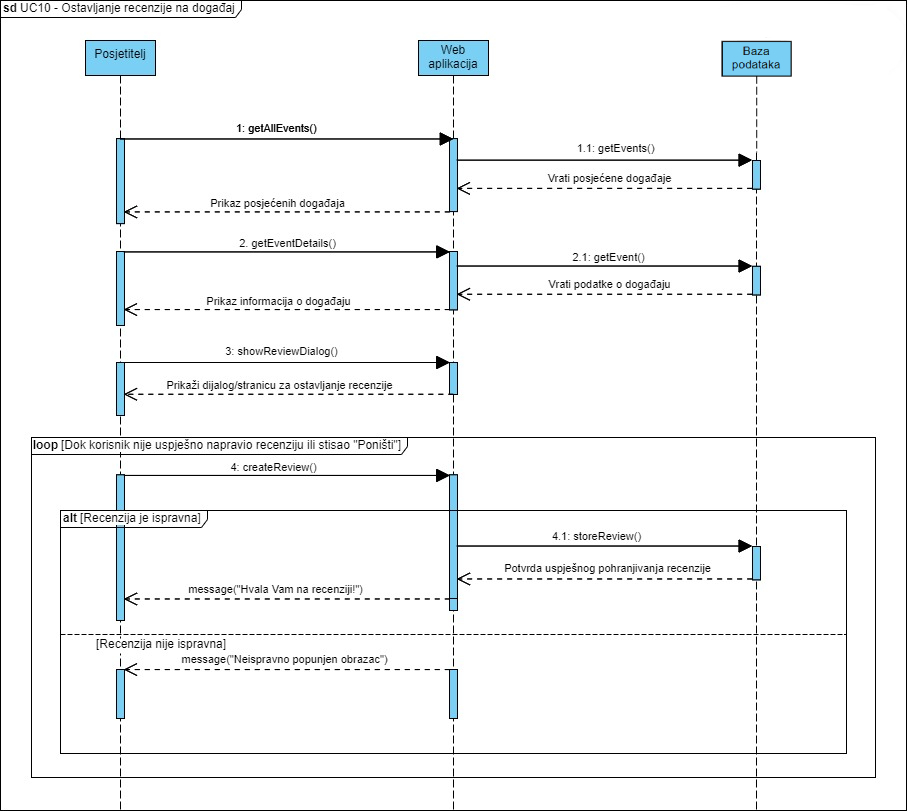
\includegraphics[width=1\textwidth]{dijagrami/seq_diagram_review.jpg}
					\caption{Sekvencijski dijagram za UC10}
				\label{fig:my_image}
				\end{figure}
				\eject
	
		\section{Ostali zahtjevi}
			%\textbf{\textit{dio 1. revizije}}\\
			% \textit{Nefunkcionalni zahtjevi i zahtjevi domene primjene dopunjuju funkcionalne zahtjeve. Oni opisuju \textbf{kako se sustav treba ponašati} i koja \textbf{ograničenja} treba poštivati (performanse, korisničko iskustvo, pouzdanost, standardi kvalitete, sigurnost...). Primjeri takvih zahtjeva u Vašem projektu mogu biti: podržani jezici korisničkog sučelja, vrijeme odziva, najveći mogući podržani broj korisnika, podržane web/mobilne platforme, razina zaštite (protokoli komunikacije, kriptiranje...)... Svaki takav zahtjev potrebno je navesti u jednoj ili dvije rečenice.}
			 
			\begin{itemize}
				\item Sustav treba omogućiti rad više korisnika u stvarnom vremenu
				\item Korisničko sučelje i sustav moraju podržavati hrvatsku abecedu (dijakritičkeznakove) pri unosu i prikazu tekstualnog sadržaja
				\item Izvršavanje dijela programa u kojem se pristupa bazi podataka ne smije trajati duže od nekoliko sekundi
				\item Sustav treba biti implementiran kao web aplikacija koristeći objektno orijentirane jezike
				\item Neispravno korištenje korisničkog sučelja ne smije narušiti funkcionalnost i rad sustava
				\item Sustav treba biti jednostavan za korištenje, korisnici se trebaju znati koristiti korisničkim sučeljem bez opširnih uputa
				\item Nadogradnja sustava ne smije narušavati postojeće funkcionalnosti sustava
				\item Sustav kao valutu koristi Euro
				\item Veza s bazom podataka mora biti kvalitetno zaštićena, brza i otporna na vanjske greške
				\item Pristup sustavu mora biti omogućen iz javne mreže pomoću HTTPS
			\end{itemize} 
			 
	
	\chapter{Arhitektura i dizajn sustava}
		%\textbf{\textit{dio 1. revizije}}\\
		%\textit{ Potrebno je opisati stil arhitekture te identificirati: podsustave, preslikavanje na radnu platformu, spremišta podataka, mrežne protokole, globalni upravljački tok i sklopovsko-programske zahtjeve. Po točkama razraditi i popratiti odgovarajućim skicama:}
	%\begin{itemize}
	%	\item 	\textit{izbor arhitekture temeljem principa oblikovanja pokazanih na predavanjima (objasniti zašto ste baš odabrali takvu arhitekturu)}
	%	\item 	\textit{organizaciju sustava s najviše razine apstrakcije (npr. klijent-poslužitelj, baza podataka, datotečni sustav, grafičko sučelje)}
	%	\item 	\textit{organizaciju aplikacije (npr. slojevi frontend i backend, MVC arhitektura) }		
	%\end{itemize}
	Arhitektura se može podijeliti na tri podsustava:
	\begin{itemize}
		\item Web poslužitelj
		\item Web aplikacija
		\item Baza podataka
	\end{itemize}

	\underline{Web Klijent} je program koji omogućuje pregled web-stranica i multimedijskih sadržaja na istima s korisničkog računala. Izvorni kod internetskih stranica se interpretira na web pregledniku i prikazuje korisniku na pristupačan način i služi kao glavna pristupna točka aplikaciji s korisničke strane. Web preglednik je također zadužen za komunikaciju s web poslužiteljem putem zahtjeva.
	
	\underline{Web poslužitelj} je program koji obrađuje zahtjeve klijenata i šalje im odgovor, time omogućavajući klijentu komunikaciju s aplikacijom. Web poslužitelj je zadužen za obradu zahtjeva i slanje odgovora putem HTTP-a (engl.\textit{Hyper Text Transfer Protocol}), standardnog protokola za prijenos informacija na webu.
	
	\underline{Web aplikacija} je program kojemu je glavna svrha pružanje funkcionalnosti i usluga korisniku putem web preglednika u obliku HTML dokumenata. Web aplikacija je izgrađena na web poslužitelju i po potrebi komunicira s bazom podataka.
	
	\underline{Baza podataka} je sustav za pohranu podataka.

	Programski jezici u kojem je web aplikacija izrađena su Python zajedno s Flask web okvirom, te JavaScript zajedno s React web okvirom. Python je interpretirani, objektno orijentirani programski jezik visoke razine. Flask je mikro web okvir za Python koji omogućuje brzo i jednostavno kreiranje web aplikacija. JavaScript je interpretirani, dinamički programski jezik visoke razine. React je JavaScript biblioteka za izgradnju korisničkih sučelja. Odabrano razvojno okruženje je Microsoft Visual Studio Code.
	Arhitektura sustava temeljiti će se na MVC arhitekturi (engl. \textit{Model-View-Controller}). MVC dozvoljava nezavisan rad na različitim dijelovima aplikacije, što omogućava brži razvoj i održavanje cijelog sustava. Njezini dijelovi su:
	\begin{itemize}
		\item \textbf{Model} - Komponenta sustava odgovorna za pohranu i dohvat podataka. Predstavljena je dinamičkim strukturama podataka. Ima interakciju s Controller-om, od kojeg prima ulazne podatke te kojemu pruža podatke za prikaz.
		\item \textbf{View} - Komponenta sustava odgovorna za prikaz podataka korisniku. Može biti formatirana u obliku HTML dokumenata, kao JSON ili u drugom formatu. Ima interakciju s Controller-om, od kojeg prima podatke za prikaz.
		\item \textbf{Controller} - Komponenta sustava koja prima ulazne podatke i prosljeđuje ih Model-u ili View-u. Zadužena je za korisničke zahtjeve i odgovore te obavlja interakciju s ostalim komponentama sustava.
	\end{itemize}

	\begin{figure}[htbp]
		\centering
		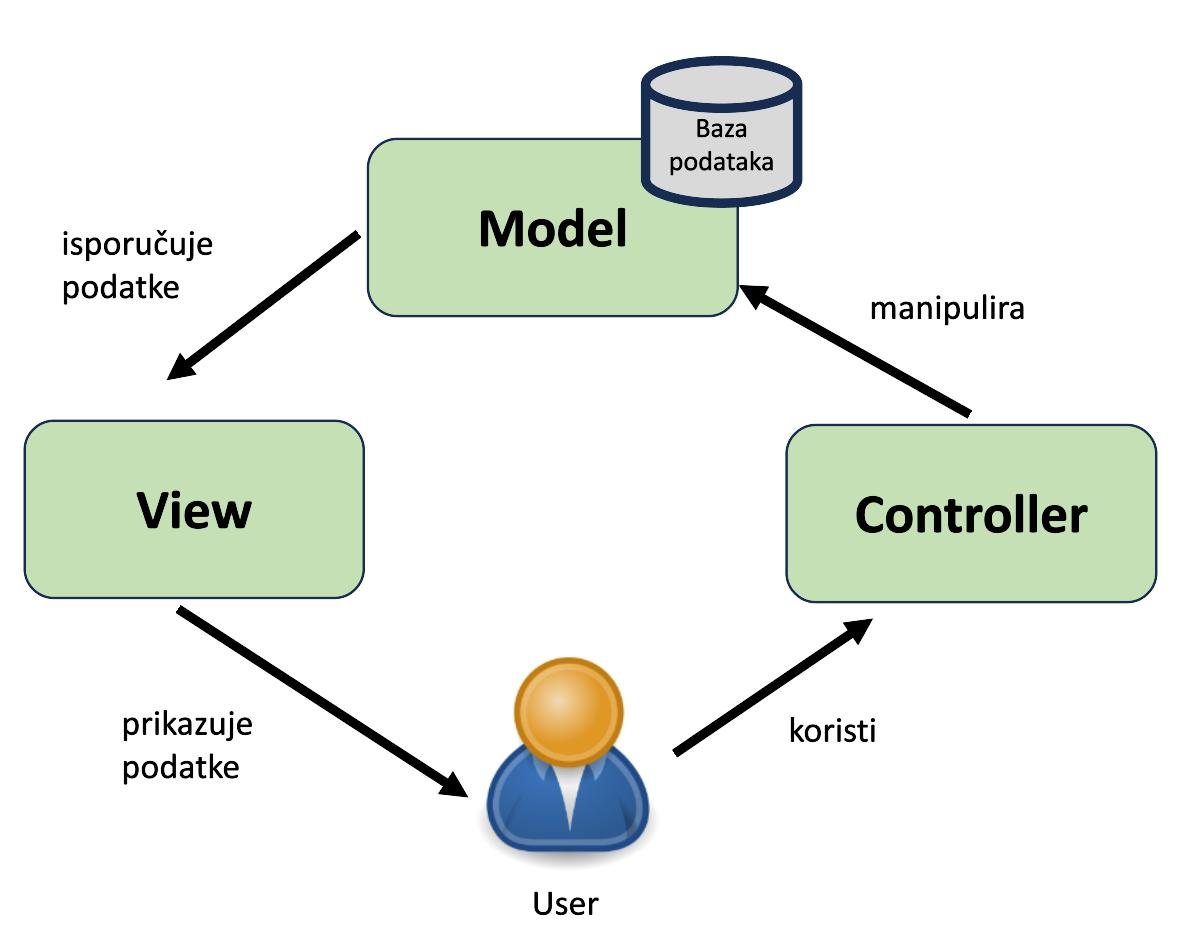
\includegraphics[width=1\textwidth]{slike/skica_mvc.jpg}
		\caption{Skica osnovne arhitekture sustava}
	\label{fig:my_image}
	\end{figure}

	%Osim navedenih dijelova arhitekture, dio poslovne logike se nalazi u sloju Service.
	

	\pagebreak
				
		\section{Baza podataka}
			
			%\textbf{\textit{dio 1. revizije}}\\
			
		%\textit{Potrebno je opisati koju vrstu i implementaciju baze podataka ste odabrali, glavne komponente od kojih se sastoji i slično.}
		
		\textrm{Za naš sustav koristit ćemo relacijsku bazu podataka čija je struktura pogodna za modeliranje stvarnog svijeta. Gradivna jedinka baze je relacija, odnosno tablica koja je definirana svojim imenom i skupom atributa. Zadaća baze podataka je brza i jednostavna pohrana, izmjena i dohvat podataka za obradu. Baza podataka naše aplikacije sastoji se od sljedećih entiteta:}
		
	\begin{packed_item}
		
		\item Račun
		\item Posjetitelj
		\item Organizator
		\item Pretplata
		\item Plaćanje
		\item Događanje
		\item Interes
		\item Recenzija
		\item Media-Događanje
		\item Država
		\item Vrsta Događanja
		\item Obavijest-Vrsta-Događanja
		\item Obavijest-Država
		\item Podatak
	\end{packed_item}
		
		
			\subsection{Opis tablica}
					

			%\textit{Svaku tablicu je potrebno opisati po zadanom predlošku. Lijevo se nalazi točno ime varijable u bazi podataka, u sredini se nalazi tip podataka, a desno se nalazi opis varijable. Svjetlozelenom bojom označite primarni ključ. Svjetlo plavom označite strani ključ}
			
			\textbf{Račun} \newline \textrm{ Ovaj entitet sadržava sve osnovne informacije o registriranom korisniku.
			Sadrži atribute: identifikator računa, korisničko ime, lozinka, e-mail, profilna slika, šifra država(ISO3), pripadna uloga.
			Ovaj entitet u vezi je \textit{One-to-One} s entitetima Posjetitelj i Organizator preko atributa accountId i u vezi \textit{Many-to-One} s entitetom Država preko atributa countryCode.}
			\begin{longtblr}[
				label=none,
				entry=none
				]{
					width = \textwidth,
					colspec={|X[6,l]|X[6, l]|X[20, l]|}, 
					rowhead = 1,
				} %definicija širine tablice, širine stupaca, poravnanje i broja redaka naslova tablice
				\hline \SetCell[c=3]{c}{\textbf{Account}}	 \\ \hline[3pt]
				\SetCell{LightGreen}accountId & INT	&  	jedinstveni identifikator računa  	\\ \hline
				username	& VARCHAR &  jedinstveni identifikator korisnika 	\\ \hline 
				eMail & VARCHAR & E-Mail korisnika  \\ \hline 
				passwordHash & VARCHAR	&  	raspršeno kriptirana lozinka korisnika	\\ \hline 
				profileImage & VARCHAR	&  	lokalna adresa na profilnu sliku korisnika	\\ \hline 
				\SetCell{LightBlue}countryCode & CHAR(3)	&  	jedinstveni id države kojoj račun pripada u formatu 3 slova (Država.countryCode) 	\\ \hline
				roleId & INT	&  	šifra uloge pridružene korisniku	\\ \hline 
			\end{longtblr}
			
			
			
			\textbf{Posjetitelj} \newline \textrm{ Ovaj entitet specijalizacija je entiteta Račun namijenjena za "obične" korisnike.
				Sadrži atribute: identifikator računa, ime i prezime.
				Ovaj entitet u vezi je \textit{One-to-One} s entitetom Račun i u
				vezi \textit{One-to-Many} s entitetima Interes, Recenzija, Opcija-Država i Opcija-Vrsta-Događanja preko atributa accountId.}
			\begin{longtblr}[
				label=none,
				entry=none
				]{
					width = \textwidth,
					colspec={|X[6,l]|X[6, l]|X[20, l]|}, 
					rowhead = 1,
				} %definicija širine tablice, širine stupaca, poravnanje i broja redaka naslova tablice
				\hline \SetCell[c=3]{c}{\textbf{Visitor}}	 \\ \hline[3pt]
				\SetCell{LightGreen}accountId & INT	&  	jedinstveni identifikator računa (Račun.accountId)  	\\ \hline
				firstName	& VARCHAR &  ime posjetitelja 	\\ \hline 
				lastName & VARCHAR & prezime posjetitelja  \\ \hline 
				
			\end{longtblr}
			
			\textbf{Organizator} \newline \textrm{ Ovaj entitet specijalizacija je entiteta Račun namijenjena za korisnike koji su organizatori.
				Sadrži atribute: identifikator računa, ime organizatora, vidljivost profila, poveznica na društvene mreže organizatora.
				Ovaj entitet u vezi je \textit{One-to-One} s entitetom Račun i u
				vezi \textit{One-to-Many} s entitetima s entitetima Plaćanje, Pretplata i Događanje preko atributa accountId.}
			\begin{longtblr}[
				label=none,
				entry=none
				]{
					width = \textwidth,
					colspec={|X[6,l]|X[6, l]|X[20, l]|}, 
					rowhead = 1,
				} %definicija širine tablice, širine stupaca, poravnanje i broja redaka naslova tablice
				\hline \SetCell[c=3]{c}{\textbf{Organizer}}	 \\ \hline[3pt]
				\SetCell{LightGreen}accountId & INT	&  	jedinstveni identifikator računa (Račun.accountId)   	\\ \hline

				organizerName	& VARCHAR &  naziv organizatora ili organizacije 	\\ \hline 
				hidden	& BOOLEAN &  zastavica koja govori o javnoj vidljivosti profila organizatora	\\ \hline 
				socials	& VARCHAR &  poveznica na društvene mreže organizatora.	\\ \hline 
									
			\end{longtblr}
			\pagebreak
			
			\textbf{Pretplata} \newline \textrm{ Ovaj entitet opisuje pretplatu koju je organizator nekad imao te koja može biti trenutno aktivna.
				Sadrži atribute: identifikator pretplate, datum početka pretplate, datum isteka pretplate, identifikator računa organizatora.
				Ovaj entitet u vezi je \textit{Many-to-One} s entitetom Organizator preko atributa accountId.}
			\begin{longtblr}[
				label=none,
				entry=none
				]{
					width = \textwidth,
					colspec={|X[6,l]|X[6, l]|X[20, l]|}, 
					rowhead = 1,
				} %definicija širine tablice, širine stupaca, poravnanje i broja redaka naslova tablice
				\hline \SetCell[c=3]{c}{\textbf{Subscription}}	 \\ \hline[3pt]
				\SetCell{LightGreen}subscriptionId & INT	&  	jedinstveni identifikator instance pretplate  	\\ \hline
				\SetCell{LightBlue}accountId & INT &  identifikator organizatora na kojeg se pretplata odnosi (Organizator.accountId) 	\\ \hline 
				startDate	& DATE &  datum početeka pretplate 	\\ \hline 
				expireDate	& DATE &  datum isteka pretplate 	\\ \hline 
			\end{longtblr}
			
			\textbf{Plaćanje} \newline \textrm{ Ovaj entitet opisuje plaćanje koje je organizator napravio prema našoj aplikaciji.
				Sadrži atribute: identifikator plaćanja, identifikator organizatora, datum plaćanja, iznos, metoda plaćanja.
				Ovaj entitet u vezi je \textit{Many-to-One} s entitetom Organizator preko atributa accountId.}
			\begin{longtblr}[
				label=none,
				entry=none
				]{
					width = \textwidth,
					colspec={|X[6,l]|X[6, l]|X[20, l]|}, 
					rowhead = 1,
				} %definicija širine tablice, širine stupaca, poravnanje i broja redaka naslova tablice
				\hline \SetCell[c=3]{c}{\textbf{Payment}}	 \\ \hline[3pt]
				\SetCell{LightGreen}paymentId & INT	&  	jedinstveni identifikator plaćanja 	\\ \hline
				\SetCell{LightBlue}accountId & INT &  identifikator organizatora na kojeg se plaćanje odnosi (Organizator.accountId) 	\\ \hline 
				date	& DATETIME &  datum i vrijeme plaćanja 	\\ \hline 
				amount	& FLOAT &  plaćen iznos 	\\ \hline 
				payment- Method	& VARCHAR &  način uplate 	\\ \hline 
			\end{longtblr}
			
			\pagebreak
			\textbf{Događanje} \newline \textrm{ Ovaj entitet opisuje događanje organizirano od strane organizatora.
				Sadrži atribute: identifikator događanja, identifikator organizatora, naziv, opis, državu, grad, lokaciju, datum i vrijeme, cijenu, naslovnu sliku događanja, 
				vrstu događanja, trajanje.
				Ovaj entitet u vezi je \textit{Many-to-One} s entitetima Organizator i Vrsta događanja preko atributa accountId i s entitetom Država preko atributa countryCode, 
				vezi \textit{One-to-Many} s entitetom Recenzija preko atributa eventId, vezi \textit{Many-to-Many} s entitetom Posjetitelj preko veze Interes i atributa eventId te u vezi \textit{One-to-Many} s entitetom Media-Događanje također preko atributa eventId.}
			\begin{longtblr}[
				label=none,
				entry=none
				]{
					width = \textwidth,
					colspec={|X[6,l]|X[6, l]|X[20, l]|}, 
					rowhead = 1,
				} %definicija širine tablice, širine stupaca, poravnanje i broja redaka naslova tablice
				\hline \SetCell[c=3]{c}{\textbf{Event}}	 \\ \hline[3pt]
				\SetCell{LightGreen}eventId & INT	&  	jedinstveni identifikator događanja 	\\ \hline
				\SetCell{LightBlue}accountId & INT &  identifikator organizatora koji organizira događanje (Organizator.accountId) 	\\ \hline 
				title	& VARCHAR &  naziv događanja 	\\ \hline 
				description	& VARCHAR &  opis događanja 	\\ \hline 
				price	& FLOAT &  cijena događanja 	\\ \hline 
				display- ImageSource	& VARCHAR &  lokalna adresa naslovne slike događanja 	\\ \hline 
				dateTime	& DATETIME &  vrijeme i datum događanja 	\\ \hline 
				countryCode	& CHAR(3) & šifra države u kojoj se događanje održava (Država.countryCode)	\\ \hline 
				city	& VARCHAR &  grad u kojem se događanje održava 	\\ \hline 
				location	& VARCHAR &  lokacija na kojoj se događanje održava	\\ \hline 
				price	& FLOAT &  cijena događanja 	\\ \hline
				duration & INTERVAL & trajanje događanja \\ \hline 
				\SetCell{LightBlue}eventType & INT &  identifikator vrste događanja (EventType.typeId)	\\ \hline
			\end{longtblr}
			
				\textbf{Interes} \newline \textrm{ Ovaj entitet predstavlja \textit{Many-to-Many} vezu interesa od strane Posjetitelja prema Događanju.
				Sadrži atribute: identifikator događanja, identifikator računa posjetitelja, stupanj zainteresiranosti.
				Ovaj entitet u vezi je \textit{Many-to-One} s entitetima Posjetitelj i Događanje preko atributa accountId i eventId.}
			\begin{longtblr}[
				label=none,
				entry=none
				]{
					width = \textwidth,
					colspec={|X[6,l]|X[6, l]|X[20, l]|}, 
					rowhead = 1,
				} %definicija širine tablice, širine stupaca, poravnanje i broja redaka naslova tablice
				\hline \SetCell[c=3]{c}{\textbf{Interest}}	 \\ \hline[3pt]
				\SetCell{LightGreen}eventId & INT	&  	indetifikator događanja na koje se interes odnosi (Događanje.eventId)	\\ \hline
				\SetCell{LightGreen}accountId & INT &  identifikator posjetitelja na kojeg se interes odnosi (Posjetitelj.accountId) 	\\ \hline 
				degreeOfInterest & INT &  stupanj interesa 	\\ \hline 
			\end{longtblr}
			
				\textbf{Recenzija} \newline \textrm{ Ovaj entitet modelira recenzije ostavljene od strane Posjetitelja za pojedina Događanja.
				Sadrži atribute: jedinstveni identifikator recenzije, identifikator događanja, identifikator računa posjetitelja, komentar, datum, vrijeme.
				Ovaj entitet u vezi je \textit{Many-to-One} s entitetima Događanje i Posjetitelj preko atributa eventId i accountId.}
			\begin{longtblr}[
				label=none,
				entry=none
				]{
					width = \textwidth,
					colspec={|X[6,l]|X[6, l]|X[20, l]|}, 
					rowhead = 1,
				} %definicija širine tablice, širine stupaca, poravnanje i broja redaka naslova tablice
				\hline \SetCell[c=3]{c}{\textbf{Review}}	 \\ \hline[3pt]
				\SetCell{LightGreen}reviewId & INT	&  	jedinstveni identifikator ostavljene recenzije	\\ \hline
				\SetCell{LightBlue}accountId & INT &  identifikator posjetitelja koji je ostavio recenziju (Posjetitelj.accountId) 	\\ \hline 
				\SetCell{LightBlue}eventId	& INT &  identifikator događanja na koje se recenzija odnosi (Događanje.eventId) 	\\ \hline 
				comment	& VARCHAR &  ostavljen komentar 	\\ \hline 
				dateTime	& DATETIME &  vrijeme i datum ostavljene recenzije 	\\ \hline 
			\end{longtblr}
			
			
			
				\textbf{Media-Događanje} \newline \textrm{ Ovaj entitet sprema lokalne adrese foto i video sadržaja koje pripada događanju.
				Sadrži atribute: jedinstveni identifikator recenzije, identifikator događanja, identifikator računa posjetitelja, komentar, datum, vrijeme.
				Ovaj entitet u vezi je \textit{Many-to-One} s entitetima Događanje i Posjetitelj preko atributa eventId i accountId.}
			\begin{longtblr}[
				label=none,
				entry=none
				]{
					width = \textwidth,
					colspec={|X[6,l]|X[6, l]|X[20, l]|}, 
					rowhead = 1,
				} %definicija širine tablice, širine stupaca, poravnanje i broja redaka naslova tablice
				\hline \SetCell[c=3]{c}{\textbf{EventMedia}}	 \\ \hline[3pt]
				\SetCell{LightGreen}mediaId & INT	&  	jedinstveni identifikator materijala	\\ \hline
				\SetCell{LightBlue}eventId	& INT &  identifikator događanja na koje se materijal odnosi (Događanje.eventId) 	\\ \hline 
				mediaType	& VARCHAR &  vrsta sadrđaja; slika ili video 	\\ \hline 
				mediaSource	& VARCHAR &  lokalna adresa sadržaja	\\ \hline 
			\end{longtblr}
			

			
			
				\textbf{Država} \newline \textrm{ Ovaj entitet modelira državu sa pripadnim šiframa i nazivom države.
				Sadrži atribute: identifikator države, sekundarni identifikator države, ime države.
				Ovaj entitet u vezi je \textit{One-to-Many} s entitetima Događanje i račun preko atributa countryCode.}
			\begin{longtblr}[
				label=none,
				entry=none
				]{
					width = \textwidth,
					colspec={|X[6,l]|X[6, l]|X[20, l]|}, 
					rowhead = 1,
				} %definicija širine tablice, širine stupaca, poravnanje i broja redaka naslova tablice
				\hline \SetCell[c=3]{c}{\textbf{Country}}	 \\ \hline[3pt]
				\SetCell{LightGreen}countryCode & CHAR(3)	&  	jedinstveni identifikator države sastavljen od 3 slova	\\ \hline
				code & CHAR(2)	&  	sekundarni jedinstveni identifikator države sastavljen od 2 slova	\\ \hline
				name & VARCHAR	&  	naziv države	\\ \hline
			\end{longtblr}

			\textbf{Vrsta Događanja} \newline \textrm{ Ovaj entitet modelira vrstu događanja koji je definiran za svako Događanje.
				Sadrži atribute: identifikator vrste, naziv vrste.
				Ovaj entitet u vezi je \textit{One-to-Many} s entitetima Događanje i Obavijest-Vrsta-Događanja preko atributa typeId.}
			\begin{longtblr}[
				label=none,
				entry=none
				]{
					width = \textwidth,
					colspec={|X[6,l]|X[6, l]|X[20, l]|}, 
					rowhead = 1,
				} %definicija širine tablice, širine stupaca, poravnanje i broja redaka naslova tablice
				\hline \SetCell[c=3]{c}{\textbf{EventType}}	 \\ \hline[3pt]
				\SetCell{LightGreen}typeId & INT	&  	jedinstveni identifikator vrste događanja	\\ \hline
				typeName & VARCHAR	&  	naziv vrste događanja	\\ \hline
			\end{longtblr}
			

			\textbf{Obavijest-Država} \newline \textrm{ Ovaj entitet sprema informaciju o tome koji korisnik ima preference za događanja u kojim državama.
			Sadrži atribute: identifikator posjetitelja, identifikator države.
			Ovaj entitet u vezi je \textit{Many-to-One} s entitetom Posjetitelj preko atributa accountId te s entitetom Država preko atributa countryCode.}
		\begin{longtblr}[
			label=none,
			entry=none
			]{
				width = \textwidth,
				colspec={|X[6,l]|X[6, l]|X[20, l]|}, 
				rowhead = 1,
			} %definicija širine tablice, širine stupaca, poravnanje i broja redaka naslova tablice
			\hline \SetCell[c=3]{c}{\textbf{NotificationCountry}}	 \\ \hline[3pt]
			\SetCell{LightGreen}accountId & INT	&  	jedinstveni identifikator posjetitelja (Posjetitelj.accountId)	\\ \hline
			\SetCell{LightGreen}countryCode & CHAR(3)	&  identifikator države (Country.countryCode). (Primarni ključ je uređeni par accountId, countryCode)	\\ \hline
		\end{longtblr}

			\textbf{Obavijest-Vrsta-Događanja} \newline \textrm{ Ovaj entitet sprema informaciju o tome koji korisnik ima preference za vrstu događanja.
			Sadrži atribute: identifikator posjetitelja, identifikator vrste događanja.
			Ovaj entitet u vezi je \textit{Many-to-One} s entitetom Posjetitelj preko atributa accountId te s entitetom Vrsta Događanja preko atributa eventType.}
		\begin{longtblr}[
			label=none,
			entry=none
			]{
				width = \textwidth,
				colspec={|X[6,l]|X[6, l]|X[20, l]|}, 
				rowhead = 1,
			} %definicija širine tablice, širine stupaca, poravnanje i broja redaka naslova tablice
			\hline \SetCell[c=3]{c}{\textbf{NotificationEventType}}	 \\ \hline[3pt]
			\SetCell{LightGreen}accountId & INT	&  	jedinstveni identifikator posjetitelja (Posjetitelj.accountId)	\\ \hline
			\SetCell{LightGreen}typeId & INT	&  identifikator vrste događanja (EventType.typeId). (Primarni ključ je uređeni par accountId, eventType)	\\ \hline
		\end{longtblr}


			\textbf{Podaci} \newline \textrm{ Ovaj entitet zadužen je spremati različite podatke potrebne za funkcioniranje i prezistenciju poslužiteljske strane.
					Sadrži atribute: naziv varijable, vrijednost varijable u string formatu.
					Ovaj entitet nije povezan s niti jednim drugim entitetom. Služi kao "look-up" tablica.}
		\begin{longtblr}[
			label=none,
			entry=none
			]{
				width = \textwidth,
				colspec={|X[6,l]|X[6, l]|X[20, l]|}, 
				rowhead = 1,
			} %definicija širine tablice, širine stupaca, poravnanje i broja redaka naslova tablice
			\hline \SetCell[c=3]{c}{\textbf{Data}}	 \\ \hline[3pt]
			\SetCell{LightGreen}entryName & VARCHAR	&  	naziv varijable	\\ \hline
			value & VARCHAR	&  vrijednost varijable u string formatu	\\ \hline
		\end{longtblr}



			\pagebreak
		\subsection{Dijagram baze podataka}
				%\textit{ U ovom potpoglavlju potrebno je umetnuti dijagram baze podataka. Primarni i strani ključevi moraju biti označeni, a tablice povezane. Bazu podataka je potrebno normalizirati. Podsjetite se kolegija "Baze podataka".}
				
				\begin{figure}[htbp]
					\centering
					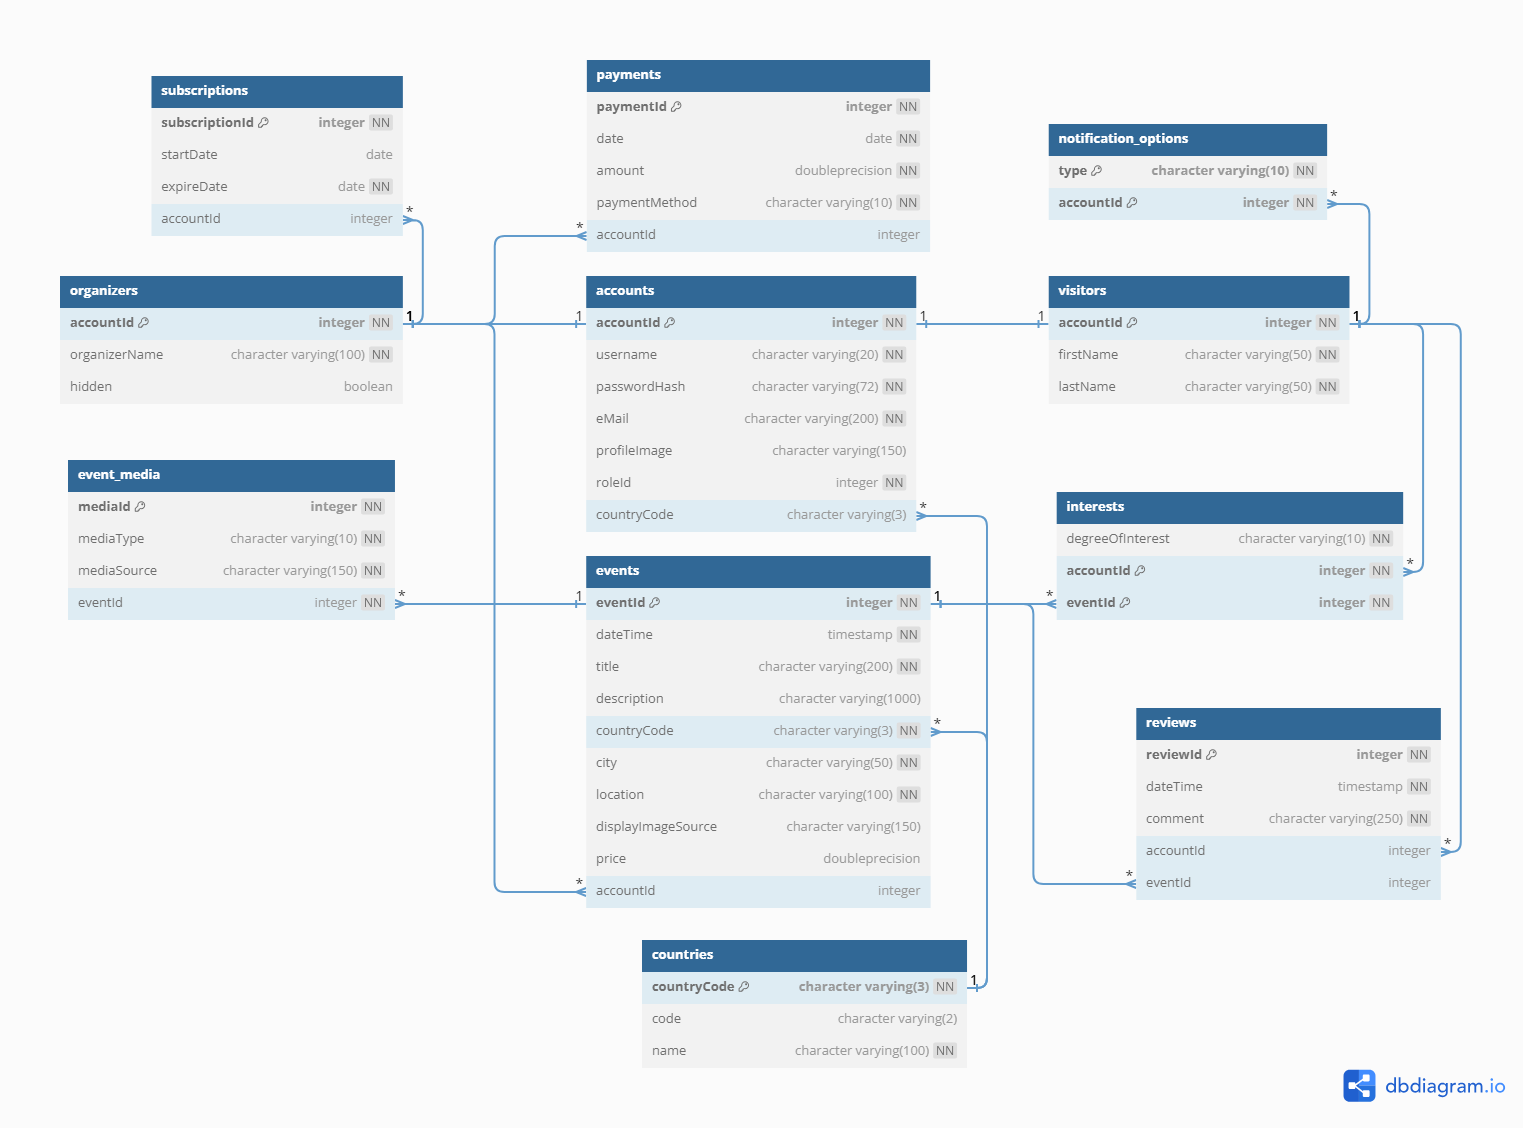
\includegraphics[width=1\textwidth]{dijagrami/relacijski_dijagram.png}
					\caption{Relacijski dijagram baze podataka}
					\label{fig:my_image}
				\end{figure}
				
				
	
			\eject
			
		\newpage	
		\section{Dijagram razreda}
		
			%\textit{Potrebno je priložiti dijagram razreda s pripadajućim opisom. Zbog preglednosti je moguće dijagram razlomiti na više njih, ali moraju biti grupirani prema sličnim razinama apstrakcije i srodnim funkcionalnostima.}\\
			%\textbf{\textit{dio 1. revizije}}\\
			%\textit{Prilikom prve predaje projekta, potrebno je priložiti potpuno razrađen dijagram razreda vezan uz \textbf{generičku funkcionalnost} sustava. Ostale funkcionalnosti trebaju biti idejno razrađene u dijagramu sa sljedećim komponentama: nazivi razreda, nazivi metoda i vrste pristupa metodama (npr. javni, zaštićeni), nazivi atributa razreda, veze i odnosi između razreda.}\\
			%\textbf{\textit{dio 2. revizije}}\\			
			%\textit{Prilikom druge predaje projekta dijagram razreda i opisi moraju odgovarati stvarnom stanju implementacije}
			
			\textit{}

			Na slikama 4.2, 4.3 i 4.4 prikazani su dijagrami razreda za podsustave u backend dijelu arhitekture. Na slici 4.3. prikazani su razredi koji nasljeđuju Controller razred. Metode tih razreda koriste Model razrede za dohvat i spremanje podataka. Metode u razredima Controller vraćaju JSON datoteke u obliku HTML status koda i podatkovnog dijela. Na slici 4.4 prikazani su Data Transfer objekti. Na slici 4.5. prikazani su razredi koji nasljeđuju Model razred i predstavljaju (modeliraju) entitete baze podataka.
			
			Zbog lakše organizacije i vidljivosti dijagrama razreda, razredi su podijeljeni u više dijagrama. Razredi su grupirani prema sličnim razinama apstrakcije i srodnim funkcionalnostima u arhitekturi MVC.
			
			\begin{figure}[htbp]
				\centering
				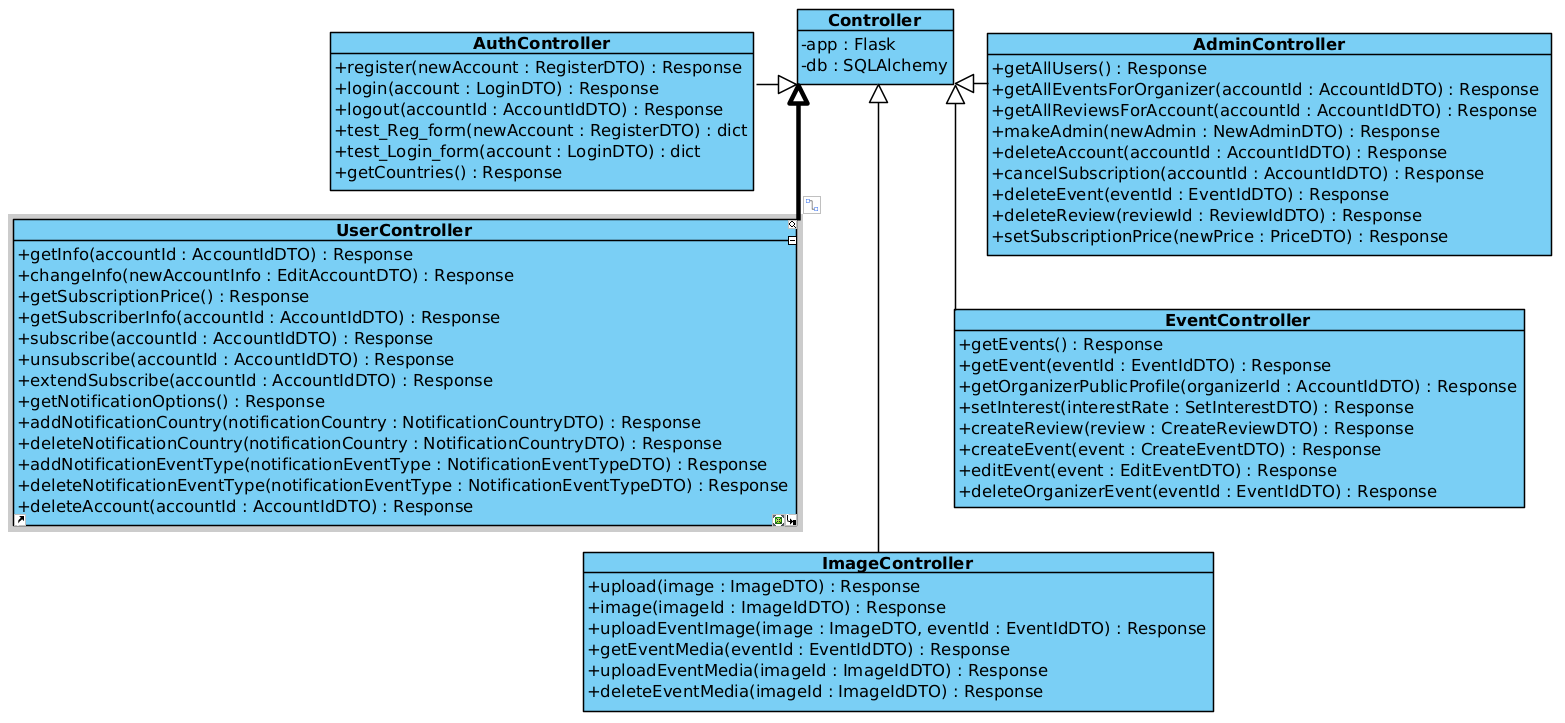
\includegraphics[width=1\textwidth]{dijagrami/dijagram_mvc_controllers.png}
				\caption{Dijagram klasa, dio Controllers}
			\label{fig:my_image}
			\end{figure}

			\newpage

			\begin{figure}[htbp]
				\centering
				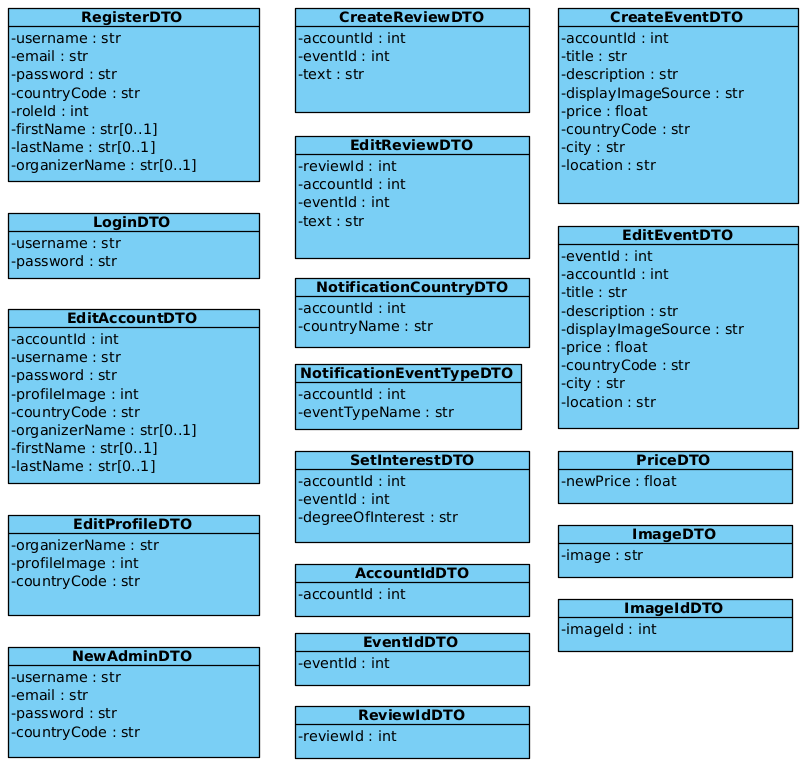
\includegraphics[width=1\textwidth]{dijagrami/dijagram_mvc_dto.png}
				\caption{Dijagram klasa, dio DTO}
			\label{fig:my_image}
			\end{figure}

			\newpage

			\begin{figure}[htbp]
				\centering
				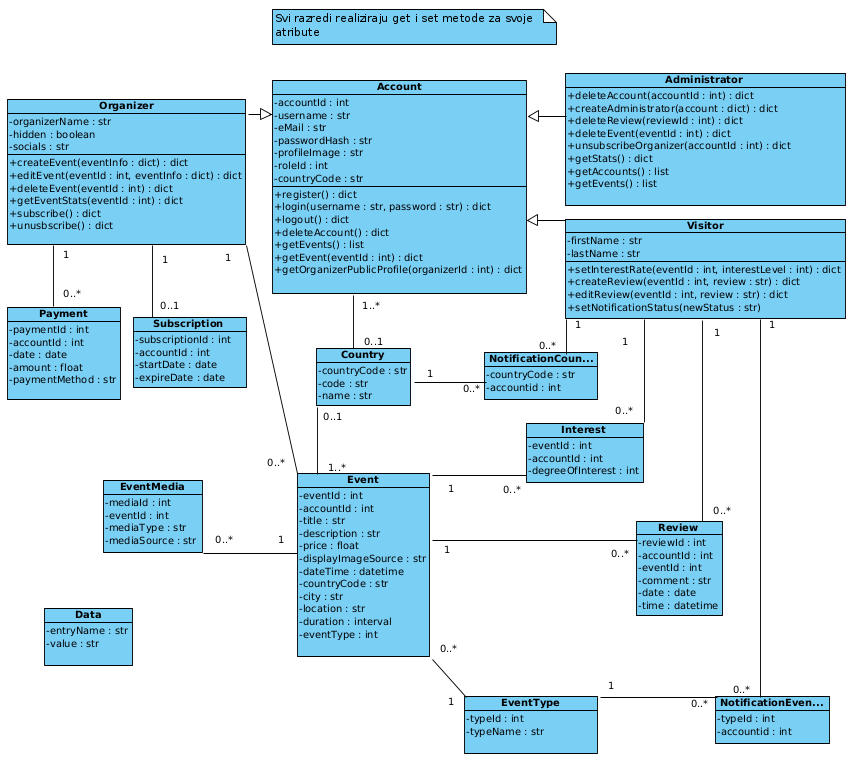
\includegraphics[width=1\textwidth]{dijagrami/dijagram_mvc_models.png}
				\caption{Dijagram klasa, dio Models}
			\label{fig:my_image}
			\end{figure}


			\eject
		
		\newpage
		\section{Dijagram stanja}
			
			% \textbf{\textit{dio 2. revizije}}\\
			
			% \textit{Potrebno je priložiti dijagram stanja i opisati ga. Dovoljan je jedan dijagram stanja koji prikazuje \textbf{značajan dio funkcionalnosti} sustava. Na primjer, stanja korisničkog sučelja i tijek korištenja neke ključne funkcionalnosti jesu značajan dio sustava, a registracija i prijava nisu. }
			Dijagram stanja opisuje dinamičko ponašanje dijela sustava.
			Prikazuje stanja objekta te prijelaze temeljene na događajima.
			Na slici 4.5 prikazan je dijagram stanja za registriranog organizatora.
			Nakon prijave, organizatoru se prikazuje početna stranica na kojoj se nalaze svi događaji.
			Klikom na "See More" gumb na pojedinom događaju, organizatoru se prikazuje kartica događaja.
			Ako je organizator vlasnik događaja, ima mogućnost uređivanja događaja.
			Na stranici postoji bočna traka koja služi za navigaciju kroz aplikaciju.
			Klikom na "Profile" organizatoru se prikazuje njegov javni profil.
			Klikom na "Account" prikazuje se stranica za pregled i uređivanje osobnih podataka te profilne slike.
			Klikom na "ConnectiNET Premium" prikazuje se stranica za upravljanje pretplatom.
			Odabirom "Create Event" organizatoru se prikazuje stranica za stvaranje novog događaja.


			\begin{figure}[htbp]
				\centering
				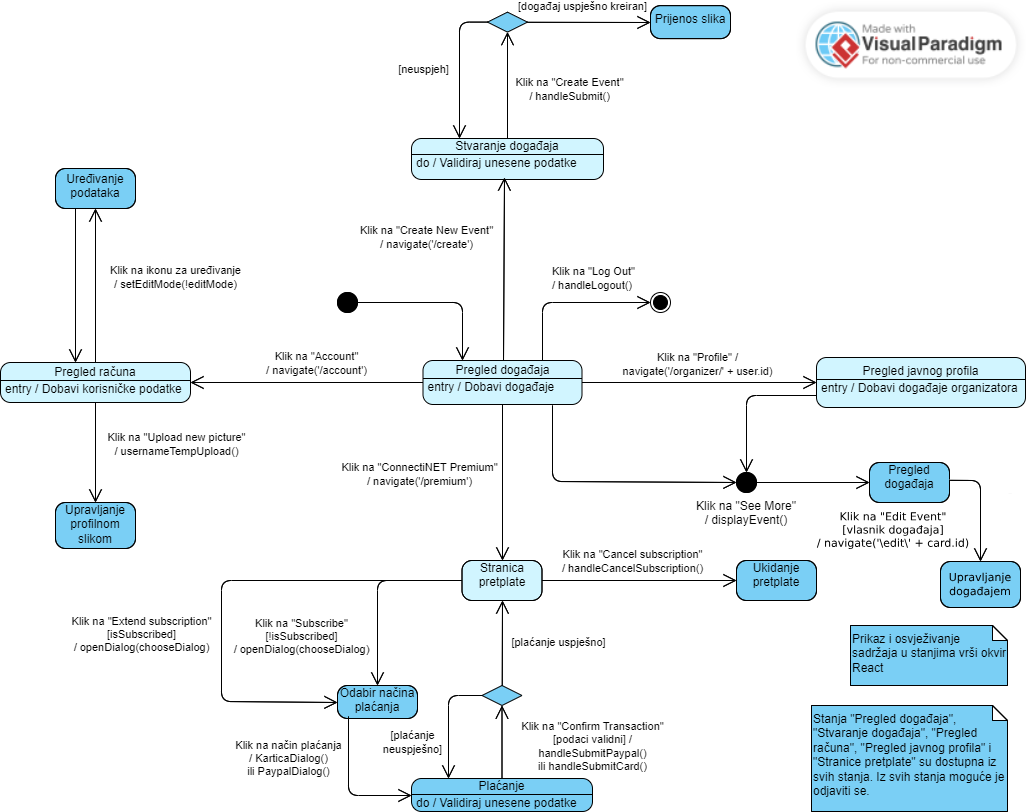
\includegraphics[width=1\textwidth]{dijagrami/dijagram_stanja.png}
				\caption{Dijagram stanja}
			\end{figure}
			
			\eject 
		
		\section{Dijagram aktivnosti}
			
			%\textbf{\textit{dio 2. revizije}}\\
			
			 %\textit{Potrebno je priložiti dijagram aktivnosti s pripadajućim opisom. Dijagram aktivnosti treba prikazivati značajan dio sustava.}\\
			 Na dijagramu aktivnosti prikazan je proces ostavljanja recenzije od strane korisnika. Korisnik se najprije prijavi u sustav ako je već jednom uspješno završio proces registracije. Nakon toga odabirom opcije pregleda događaja dolazi do popisa svih trenutno evidentiranih događaja u bazi podataka nad kojim odabirom neke od funkcija za kontrolu pregleda (sortiranje, filtriranje, traženje ključne riječi) reducira izbor prema vlastitim željama. Kada pronađe i odabere željeni događaj otvara mu se prikaz s dodatnim informacijama o dotičnom događaju. Ako je događaj završio unazad 48 sati, Korisnik odabirom funkcije za ostavljenje recenzija popunjava obrazac za ostavljanje recenzije. Ispravnim popunjavanjem obrasca, recenzija se pohranjuje u bazi podataka.  
			 \begin{figure}[htbp]
				\centering
				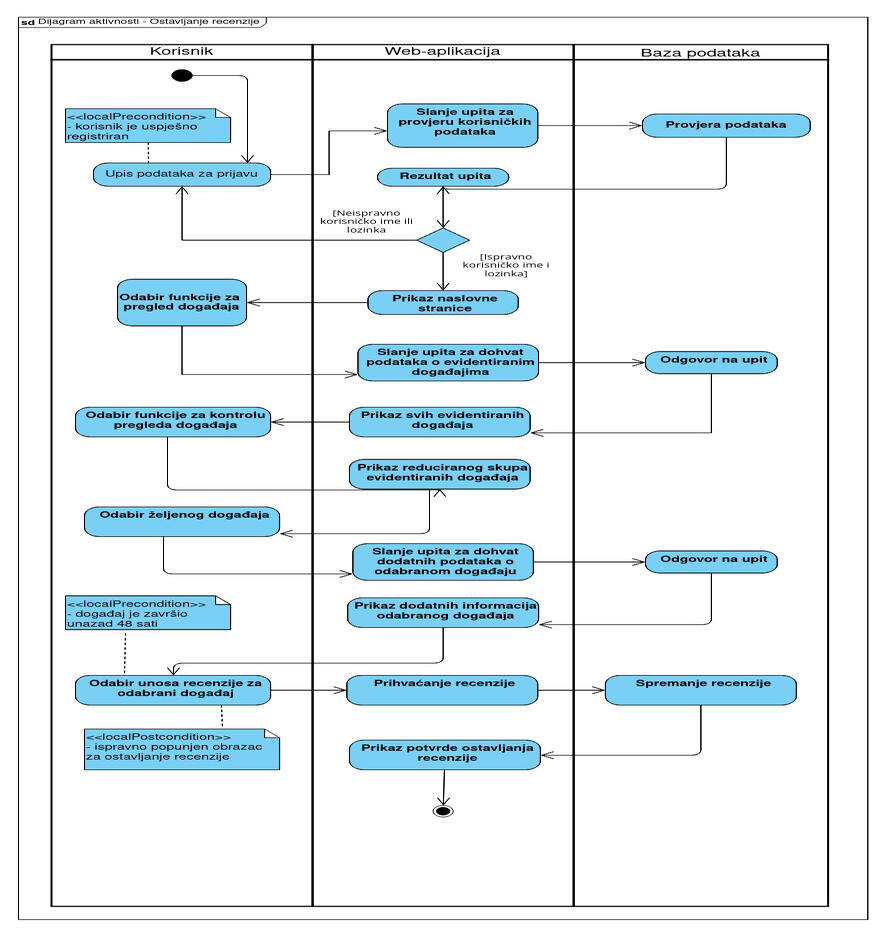
\includegraphics[width=1\textwidth]{dijagrami/diagram_aktivnosti_finally.jpeg} %height=0.7\textheight
				\caption{Dijagram aktivnosti}
			\label{fig:my_image}
			\end{figure}

			\eject
		\section{Dijagram komponenti}
		
			%\textbf{\textit{dio 2. revizije}}\\
		
			 %\textit{Potrebno je priložiti dijagram komponenti s pripadajućim opisom. Dijagram komponenti treba prikazivati strukturu cijele aplikacije.}
			 Sustavu se pristupa preko dva različita sučelja. Preko sučelja za dohvat HTML, CSS, JS i JSX datoteka poslužuju se datoteke koje pripadaju frontend dijelu aplikacije. Router je komponenta koja na upit s url-a određuje koja datoteka će se poslužiti na sučelje. Frontend dio se sastoji od većeg broja JavaScript datoteka koje su raspoređene u logičke cjeline views, ui i context. Views datoteke definiraju osnovnu strukturu stranice koja će se prikazati korisniku. Ui datoteke predstavljaju komponente koje dopunjuju strukturu stranice. Context sadrži kontekste koji olakšavaju dijeljenje podataka između React komponenata. ProtectedComponent.jsx datoteka je React komponenta koja služi kao zaštitni omotač za druge komponente. Koristi se za provjeru je li korisnik prijavljen i ima li odgovarajuće ovlasti za pristup određenim dijelovima aplikacije. Ako korisnik nije prijavljen ili nema odgovarajuće ovlasti, komponenta preusmjerava korisnika na stranicu za prijavu ili na drugu stranicu. Sve JavaScript datoteke ovise o React biblioteci iz koje dohvaćaju gotove komponente kao što su gumbi, forme i slično. Preko sučelja za dohvat JSON podataka pristupa se REST API komponenti. REST API poslužuje podatke koji pripadaju backend dijelu aplikacije. SQLAlchemy je zadužen za dohvaćanje tablica iz baze podataka pomoću SQL upita. Podaci koji su pristigli iz baze se šalju dalje MVC arhitekturi u obliku jednostavnih Python klasa ili tuple-ova koji se kasnijom obradom pretvaraju u JSON objekte. Util.py implementira sučelje koje se koristi za provjeru prava pristupa određenim podacima i rutama. React-view komponenta preko oba sučelja komunicira s ConnectiNET aplikacijom te ovisno o korisnikovim akcijama osvježava prikaz i dohvaća nove podatke ili datoteke. Oba sučelja ovise o komponenti DataController.js koja preuzetim zahtjevima s korisničkog sučelja dodaje potrebne parametre i šalje zahtjev na poslužitelj. Kada poslužitelj vrati odgovor, DataController.js obrađuje taj odgovor i prosljeđuje ga natrag korisničkom sučelju.
			 \begin{figure}[htbp]
				\centering
				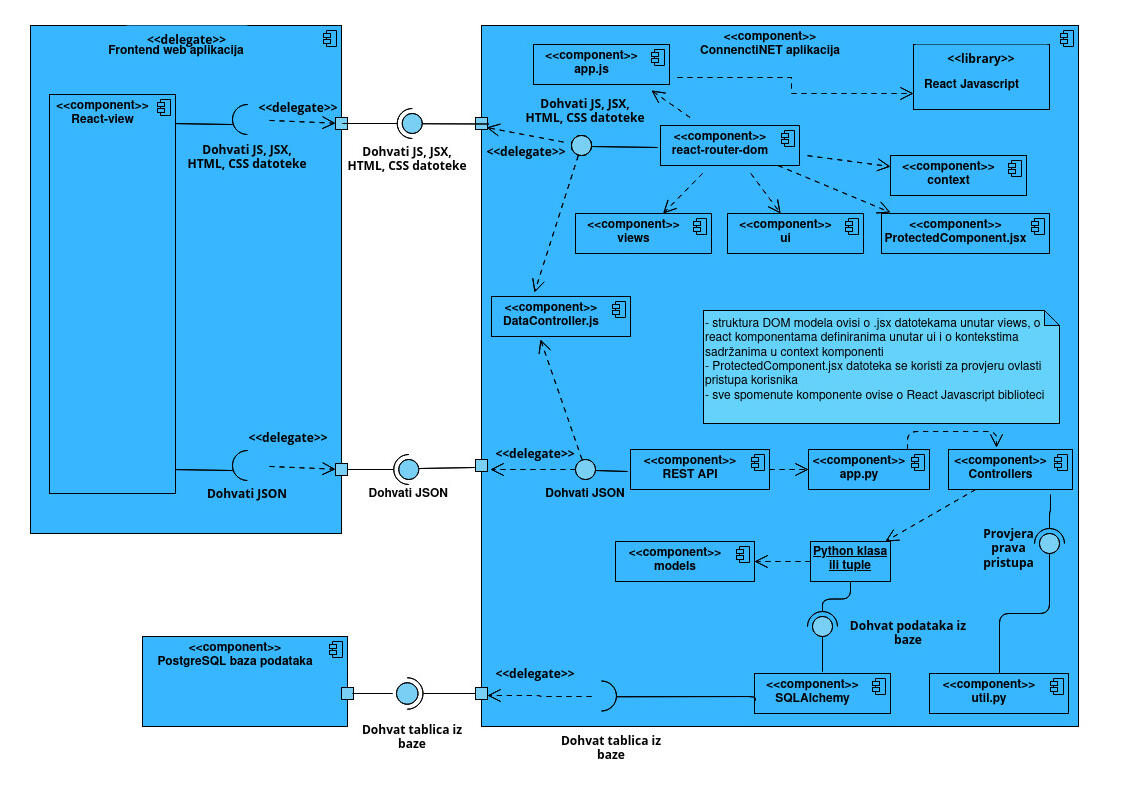
\includegraphics[width=1\textwidth]{dijagrami/component_diagram_finally.jpeg}
				\caption{Dijagram komponenti}
			\label{fig:my_image}
			\end{figure}
	\chapter{Implementacija i korisničko sučelje}
		
		
		\section{Korištene tehnologije i alati}
		
			%\textbf{\textit{dio 2. revizije}}
			 Komunikacija u timu realizirana je korištenjem aplikacije Discord\footnote{https://discord.com/}, a kao sustav za upravljanje izvornim kodom Git\footnote{https://git-scm.com/}. Za izradu UML dijagrama korišten je alat VisualParadigm\footnote{https://online.visual-paradigm.com/}. Udaljeni repozitorij projekta je dostupan na web platformi GitHub\footnote{https://github.com/}.
			 
			 Kao uređivač izvornog koda korišten je Visual Studio Code\footnote{https://code.visualstudio.com/} napravljen od strane Microsofta s Electron Frameworkom, za Windows, Linux i macOS. Dolazi s ugrađenom podrškom za JavaScript, TypeScript i Node.js te ima bogat ekosustav proširenja za druge jezike i runtimeove. Neke od značajki uključuju podršku za debugiranje, isticanje sintakse, inteligentno dovršavanje koda, isječke, refaktoriranje koda i ugrađeni Git.
			 
			 Za modeliranje baze podataka korišten je web alat ERDPlus\footnote{https://erdplus.com/} koji između ostalog omogućuje jednostavno stvaranje ER dijagrama i relacijskih shema. Ovaj besplatan alat pruža pomoć u vizualizaciji i efikasnom dizajniranju baza podataka pomoću automatskog generiranja SQL DDL (Data Definition Language) izjava na temelju korisnički unesenih shema.
             
			 Od sustava za upravljanje bazama podataka korišten je PostgreSQL\footnote{ https://www.postgresql.org/}. Sustav poštuje ACID principe pri izvođenju transakcija, proširljiv je i drži se većine SQL:2011 standarda.
			 
			 Aplikacija je napisana koristeći web okvir Flask\footnote{https://flask.palletsprojects.com/en/3.0.x/}. Razvijen je od strane Armina Ronachera, vođe Međunarodne grupe entuzijasta za Python. Temelji se na WSGI alatima i Jinja2 predlošku. Ovaj okvir pokriva širok spektar primjene, od osnovnih koncepta kao što su postavljanje i instalacija do naprednijih koncepta poput autentifikacije korisnika i integracije baze podataka.
			 
			 Za izradu frontenda korišten je React\footnote{https://reactjs.org/} i jezik JavaScript\footnote{https://www.javascript.com/}. React, također poznat kao React.js ili ReactJS, je biblioteka u JavaScriptu za izgradnju korisničkih sučelja. Održavana je od strane Facebooka. React se najčešće koristi kao osnova u razvoju web ili mobilnih aplikacija. Složene aplikacije u Reactu obično zahtijevaju korištenje dodatnih biblioteka za interakciju s API-jem.

			 Kao pomoć u razvoju korištena je usluga ElephantSQL\footnote{https://www.elephantsql.com/} za hosting baze podataka. ElephantSQL nudi korisnički prijateljsku i skalabilnu platformu za upravljanje PostgreSQL bazama podataka u oblaku. Pojednostavljuje proces opskrbe, upravljanja i skaliranja PostgreSQL instanci, omogućujući razvojnom timu da se usredotoči na funkcionalnost svoje aplikacije umjesto na upravljanje infrastrukturom.

			 S ciljem pojednostavljenja procesa slanja e-mailova koji je integriran unutar aplikacije, korišten je Mailjet\footnote{https://www.mailjet.com/} - cloud-based pružatelj usluga e-pošte (ESP) koji omogućuje slanje transakcijskih i marketinških e-mail kampanja. Mailjetova platforma osigurava pouzdano slanje na sigurnoj i robustnoj infrastrukturi koja se nalazi na Google Cloud Platformi, te nadzire i optimizira ključne analitike poput stopa otvaranja, stopa odbijanja i spam pogodaka.

			 Za pohranu slika korišten je Firebase Storage\footnote{https://firebase.google.com/products/storage/} - usluga koja dio platforme Firebase unutar Google Cloud Platform-a (GCP) i koja omogućuje pohranu i upravljanje medijima generiranim od strane korisnika web i mobilnih aplikacija. Kada koristimo Firebase Storage, datoteke se prenose izravno od i do klijenta. Kada korisnik prenese datoteku na Firebase Storage, generira se URL za tu datoteku. Taj URL se može zatim spremiti u bazu podataka na poslužitelju. Dakle, na poslužitelju ostaje samo poveznica na datoteku, a sama datoteka se pohranjuje u Firebase Storage. Ovo omogućuje efikasno upravljanje datotekama bez potrebe za velikom infrastrukturom na poslužitelju. Također, smanjuje se opterećenje na poslužitelju jer se prijenos datoteka obavlja izravno između klijenta i Firebase Storage-a.

			 Svoju primjenu u izradi ovog projekta pronašao je i Docker\footnote{https://www.docker.com/} - otvorena platforma za razvoj, isporuku i pokretanje aplikacija. Docker omogućuje odvajanje aplikacija od infrastrukture kako bi se softver mogao brzo isporučiti1. Docker pruža mogućnost pakiranja i pokretanja aplikacije u labavo izoliranom okruženju zvanom kontejner. Kontejneri su lagani i sadrže sve što je potrebno za pokretanje aplikacije. U kontekstu izrade web aplikacija, Docker pojednostavljuje razvoj omogućujući programerima stvaranje prijenosnih i konzistentnih okruženja aplikacija, smanjujući složenost postavljanja i održavanja razvojnih, testnih i produkcijskih okruženja. Kontejneri su odlični za kontinuiranu integraciju i kontinuiranu isporuku (CI/CD) radnih tokova.

             Kao platforma za puštanje u pogon korišten je Render\footnote{https://render.com/} koji omogućuje brzo i jednostavno postavljanje web aplikacija. Podržava sve glavne jezike, besplatne certifikate, zaštitu od DDoS napada i automatsko postavljanje iz GitHuba. Također nudi i sučelje za brzo i jednostavno objavljivanje statičkog web sadržaja. Može se koristiti za postavljanje različitih vrsta aplikacija, uključujući Node.js, Express i Flask aplikacije.		 
			 
			 Za izradu dokumentacije korišten je LateX\footnote{https://www.latex-project.org/}, markup jezik koji svoju osnovnu primjenu nalazi u izradi znanstvenih publikacija. Osnovna mu je značajka da pisac koristi konvencije označavanja koje predstavljaju ugrađene naredbe za definiranje opće strukture dokumenta, stiliziranje teksta, dodavanje citata, unakrsnih referenci i sl.Tako stvorenu LaTeX datoteku obrađuje softver zvan TeX engine koji koristi ugrađene naredbe kako bi vodio i kontrolirao proces izgradnje profesionalno složenenog PDF dokumenta.
			\eject 
		
	
		\section{Ispitivanje programskog rješenja}
			
			
			\subsection{Ispitivanje komponenti}
			Svi testovi komponenti su izvršeni koristeći python biblioteke unittest i requests. Ispitivanje se radilo po obrascima uporabe kako bi se provjerila osnovna funkcionalnost sustava i neki rubni slučajevi, pokut pokušaja dohvata bez tokena za autorizaciju. Prikazano je ispitivanje UC2, UC5, UC6, UC12 i UC13. Slijedi izvorni kod datoteke za testiranje, također vidljiv u /testing direktoriju repozitorija koda. Ispod izvornog koda je i slika izlaza terminala nakon pokretanja testiraanja.

			\begin{verbatim}
				import requests
				import unittest

				class TestApp(unittest.TestCase):
					def setUp(self):
						self.base_url = 'http://127.0.0.1:5000'
						
					def test_login(self, username, password):
						response = requests.post(
							self.base_url + '/login', 
							json={'username': username, 'password': password}
						)
						self.assertEqual(response.status_code, 200, 'Status code is not 200')
						self.assertIn(
							'access_token', 
							response.json()['data'], 
							'Response does not contain access_token'
						)
						print('Test Login Passed')
						return response.json()

					def test_get_events(self, token):
						response = requests.get(
							self.base_url + '/getEvents', 
							headers={'Authorization': 'Bearer ' + token}
						)
						self.assertEqual(
							response.status_code, 
							200, 
							'Status code is not 200'
						)
						self.assertIsInstance(
							response.json()['data'], 
							list, 
							'Response data is not a list'
						)
						print('Test Get Events Passed')
						return response.json()
					
					def test_get_events_without_token(self):
						response = requests.get(self.base_url + '/getEvents')
						self.assertEqual(
							response.status_code, 
							401, 
							'Status code is not 401'
						)
						self.assertIn(
							'msg', 
							response.json(), 
							'Response does not contain msg'
						)
						print('Test Get Events Without jwt failed, as expected')
						return response.json()
					
					def test_create_event(self, token):
						response = requests.post(
							self.base_url + '/api/createEvent', 
							headers={'Authorization': 'Bearer ' + token}, 
							json={
								'title':'EventName',
								'description':'Description',
								'city':'City',
								'location':'Place',
								'countryCode':'CCK',
								'eventType':'Concert',
								'dateTime':'2024-01-26T12:00',
								'duration':'2024-01-29T12:00',
								'price':'1'
							})
						self.assertEqual(
							response.status_code, 200, 
							'Status code is not 200'
						)
						self.assertIn(
							'eventId', 
							response.json()['data'], 
							'Response does not contain eventId'
						)
						print('Test Edit Event Passed')
						return response.json()
					
					def test_edit_event(self, token, id):
						response = requests.put(
							self.base_url + '/api/editEvent/62', 
							headers={'Authorization': 'Bearer ' + token},
							json={
								'title':'NewEventName',
								'description':'New Description',
								'city':'New City',
								'location':'New Place',
								'countryCode':'HRV',
								'eventType':'Community',
								'dateTime':'2025-01-26T12:00',
								'duration':'2025-02-29T12:00',
								'price':'20'
							})
						self.assertEqual(
							response.status_code, 
							200, 
							'Status code is not 200'
						)
						self.assertIn(
							'success', 
							response.json(), 
							'Response does not contain success'
						)
						print('Test Edit Event Passed')
						return response.json()
					
					def test_delete_account(self, token):
						response = requests.delete(
							self.base_url + '/api/deleteAccount', 
							headers={'Authorization': 'Bearer ' + token}
						)
						self.assertEqual(
							response.status_code, 
							200, 
							'Status code is not 200'
						)
						self.assertIn(
							'success', 
							response.json(), 
							'Response does not contain success'
						)
						print('Test Delete Account Passed')
						return response.json()
					
					

				# Instantiate the test class
				test_app = TestApp()
				test_app.setUp()

				# Login
				jwt = test_app.test_login(
					'kraljevi', 
					'pass123kraljevi')['data']['access_token']

				# Attempt to get events
				test_app.test_get_events(jwt)
				test_app.test_get_events_without_token()

				# Create and edit an event
				new_event_id = test_app.test_create_event(
					jwt)['data']['eventId']
				test_app.test_edit_event(jwt, new_event_id)

				# Delete a user
				jwt = test_app.test_login('testuser', 
					'password123')['data']['access_token']
				test_app.test_delete_account(jwt)
			\end{verbatim}			
			\begin{figure}[htbp]
				\centering
				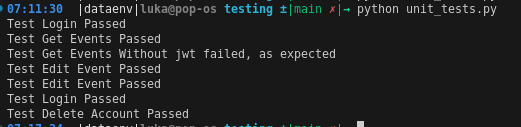
\includegraphics[width=1\textwidth]{slike/unit_test.png}
				\caption{Izlaz terminala nakon pokretanja testiranja}
			\label{fig:my_image}
			\end{figure}
			
			\subsection{Ispitivanje sustava}
			Svi testovi izvršeni su koristeći Selenium WebDriver. Ispitivanje se radilo po obrascima uporabe kako bi se provjerila osnovna funkcionalnost sustava. Prikazano je ispitivanje UC1 (i UC2), UC4, UC5, UC9 i UC12. Izvorni kod vidljiv je u direktoriju testing.
			
			\noindent \underbar{\textbf{Ispitni slučaj 1: Stvaranje korisničkog računa}}
			\begin{packed_item}

				\item  \textbf{Ulaz:}
				\item[] \begin{packed_enum}

					\item Otvaranje stranice za registraciju u web pregledniku
					\item Unos uloge, imena, prezimena, korisničkog imena, email adrese, lozinke i države
					\item Odabir opcija "Sign Up" i "Sign In"

				\end{packed_enum}
				
				\item  \textbf{Očekivani rezultat:}
				\item[] \begin{packed_item}
				\item[1] Uneseni podaci su vidljivi na stranici za prijavu
				\item[2.a] Korisnik je uspješno registriran
				\item[2.b] Neki od unesenih podataka je u neispravnom formatu, obavijest upozorava korisnika
				\end{packed_item}

				\item  \textbf{Rezultat:} Svi očekivani rezultati su ostvareni i provjereni uspješnom prijavom na kreirani korisnički račun. Aplikacija je prošla test.

				\begin{figure}[htbp]
					\centering
					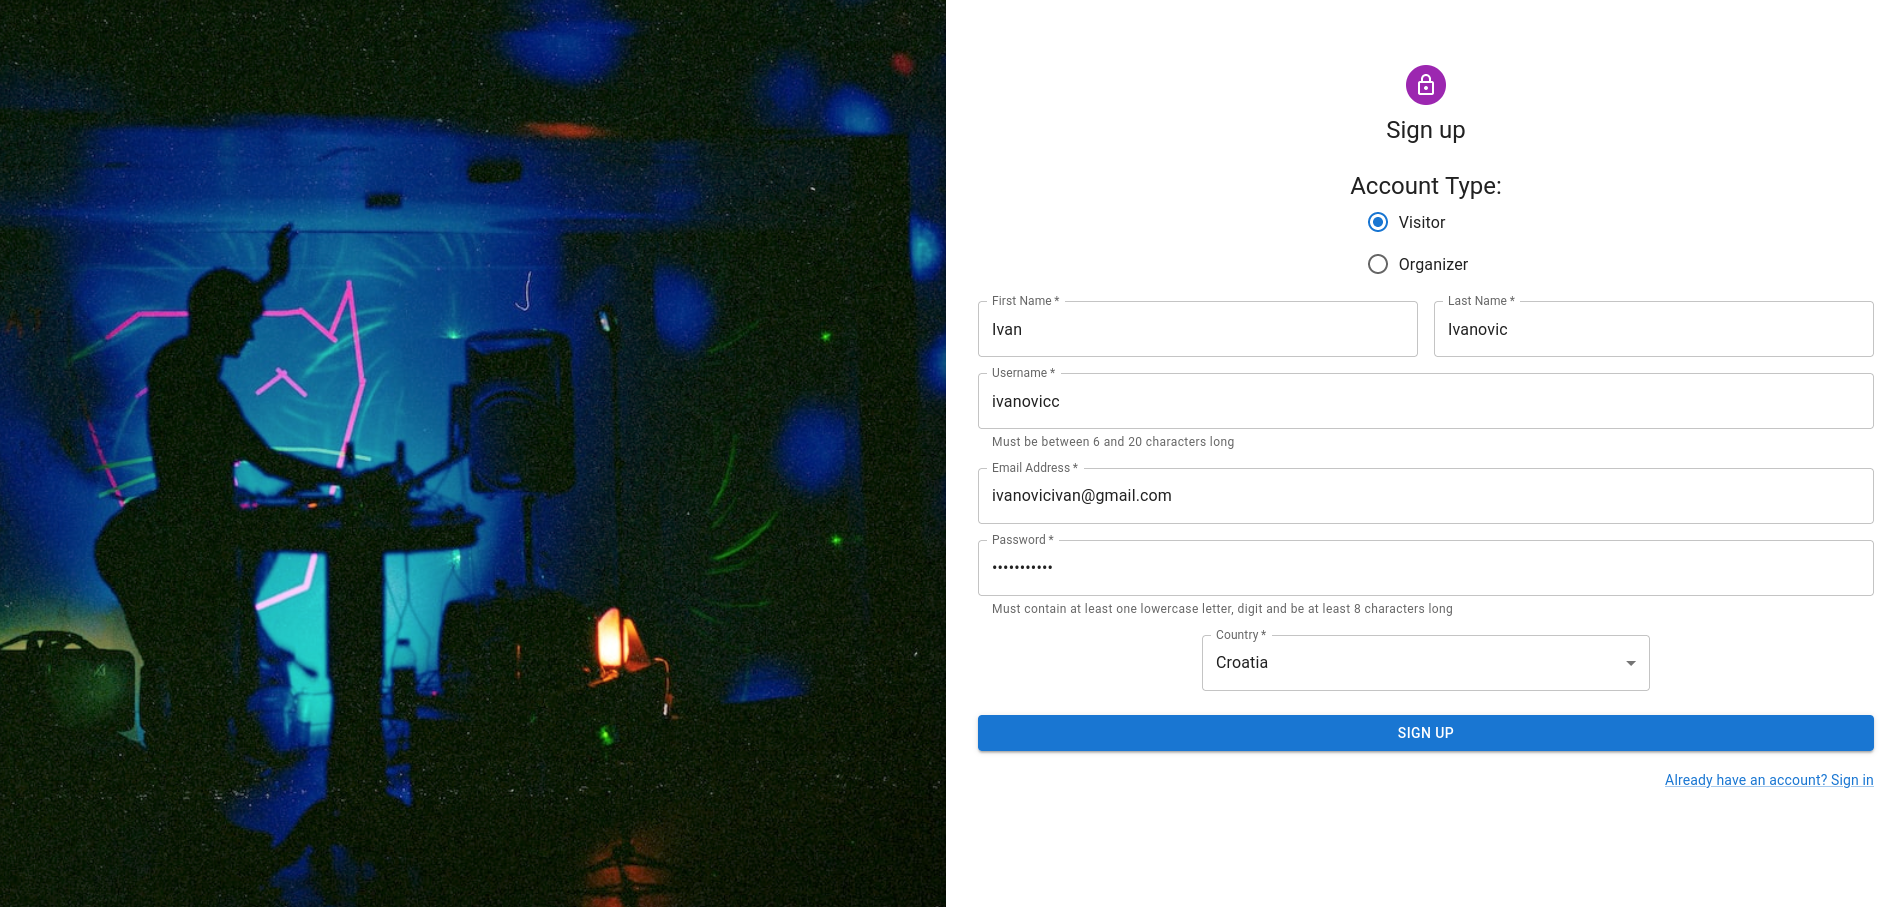
\includegraphics[width=1\textwidth]{slike/selenium_test_1.png}
					\caption{Testiranje stvaranja korisničkog računa}
				\label{fig:my_image}
				\end{figure}
			\end{packed_item}

			\noindent \underbar{\textbf{Ispitni slučaj 2: Uređivanje korisničkog računa}}
			\begin{packed_item}

				\item  \textbf{Ulaz:}
				\item[] \begin{packed_enum}

					\item Otvaranje Account stranice u web pregledniku
					\item Odabir opcije "Edit Account" i "Save Changes"
					\item Unos novih podataka u polja za uređivanje

				\end{packed_enum}
				
				\item  \textbf{Očekivani rezultat:}
				\item[] \begin{packed_item}
				\item[1] Uneseni podaci su vidljivi na stranici za uređivanje
				\item[2.a] Korisnik je uspješno uređen
				\item[2.b] Neki od unesenih podataka je u neispravnom formatu, obavijest upozorava korisnika
				\end{packed_item}

				\item  \textbf{Rezultat:} Svi očekivani rezultati su ostvareni. Aplikacija je prošla test.

				\begin{figure}[htbp]
					\centering
					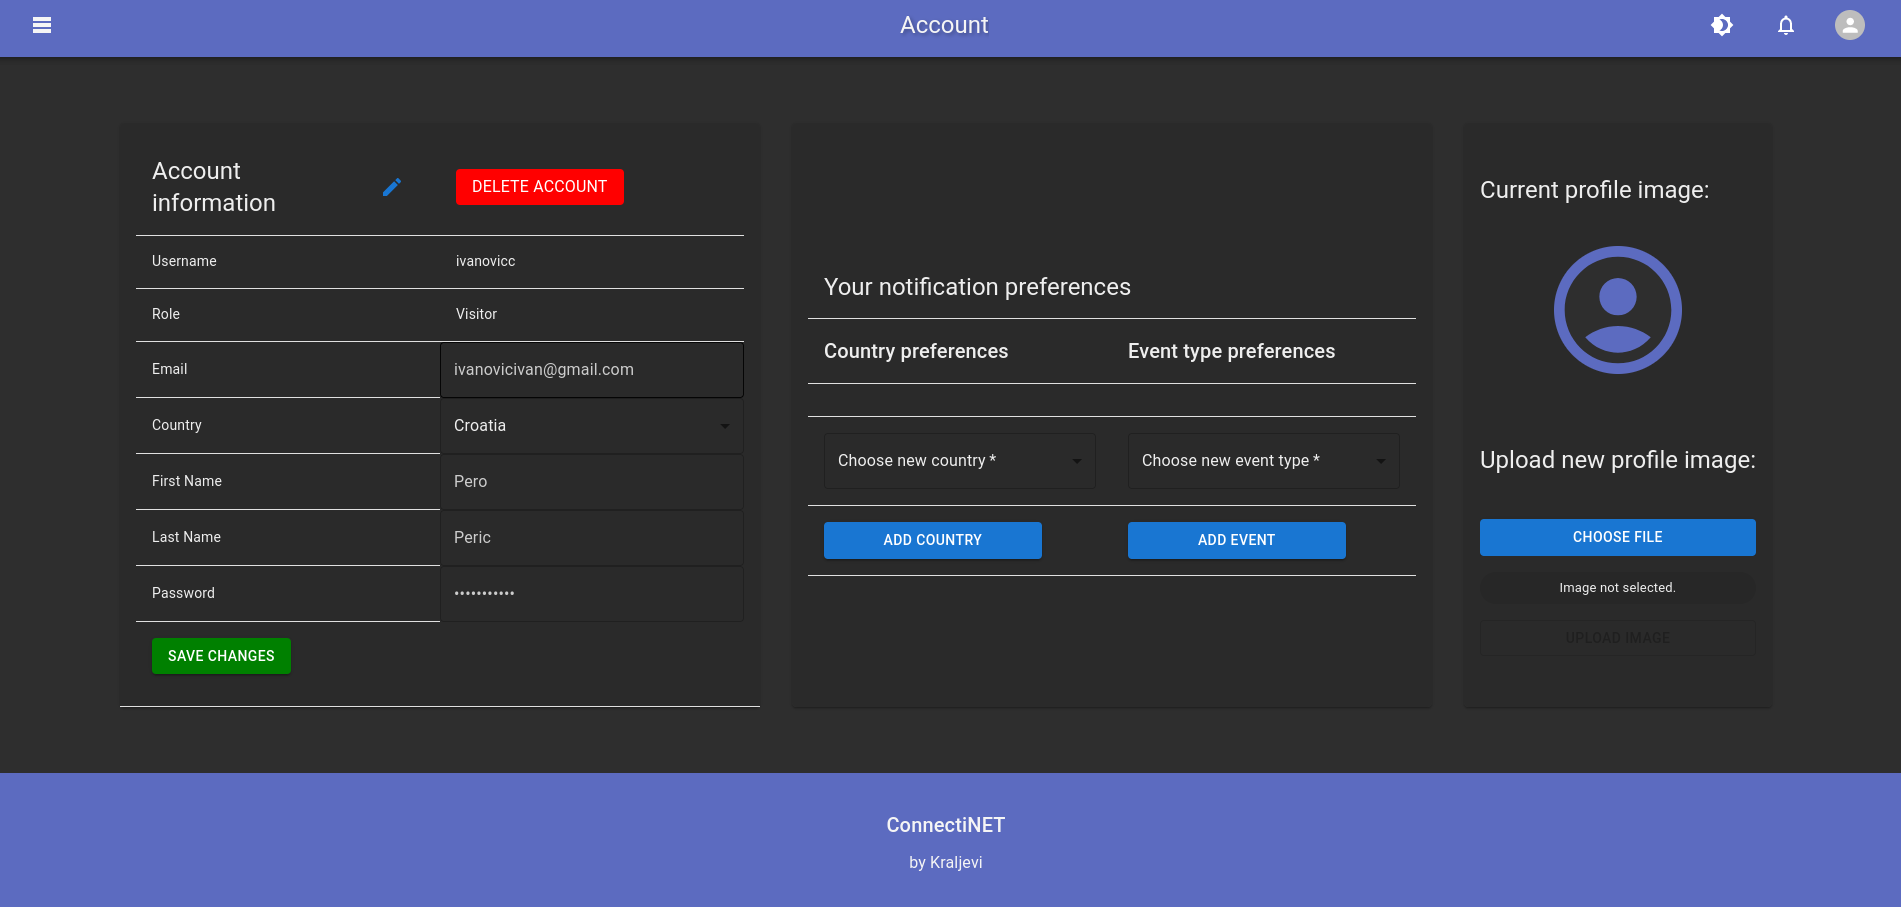
\includegraphics[width=1\textwidth]{slike/selenium_test_2.png}
					\caption{Testiranje uređivanja korisničkog računa}
				\label{fig:my_image}
				\end{figure}
			\end{packed_item}

			\noindent \underbar{\textbf{Ispitni slučaj 3: Brisanje korisničkog računa}}
			\begin{packed_item}

				\item  \textbf{Ulaz:}
				\item[] \begin{packed_enum}

					\item Otvaranje Account stranice u web pregledniku
					\item Odabir opcije "Delete Account" i potvrde brisanja

				\end{packed_enum}
				
				\item  \textbf{Očekivani rezultat:}
				\item[] \begin{packed_item}
				\item[1.a] Korisnički račun je obrisan nakon pritiska "Yes" za potvrdu brisanja
				\item[1.b] Korisnički račun nije obrisan nakon pritiska "No" za potvrdu brisanja 
				\end{packed_item}

				\item  \textbf{Rezultat:} Svi očekivani rezultati su ostvareni. Aplikacija je prošla test.
				\begin{figure}[htbp]
					\centering
					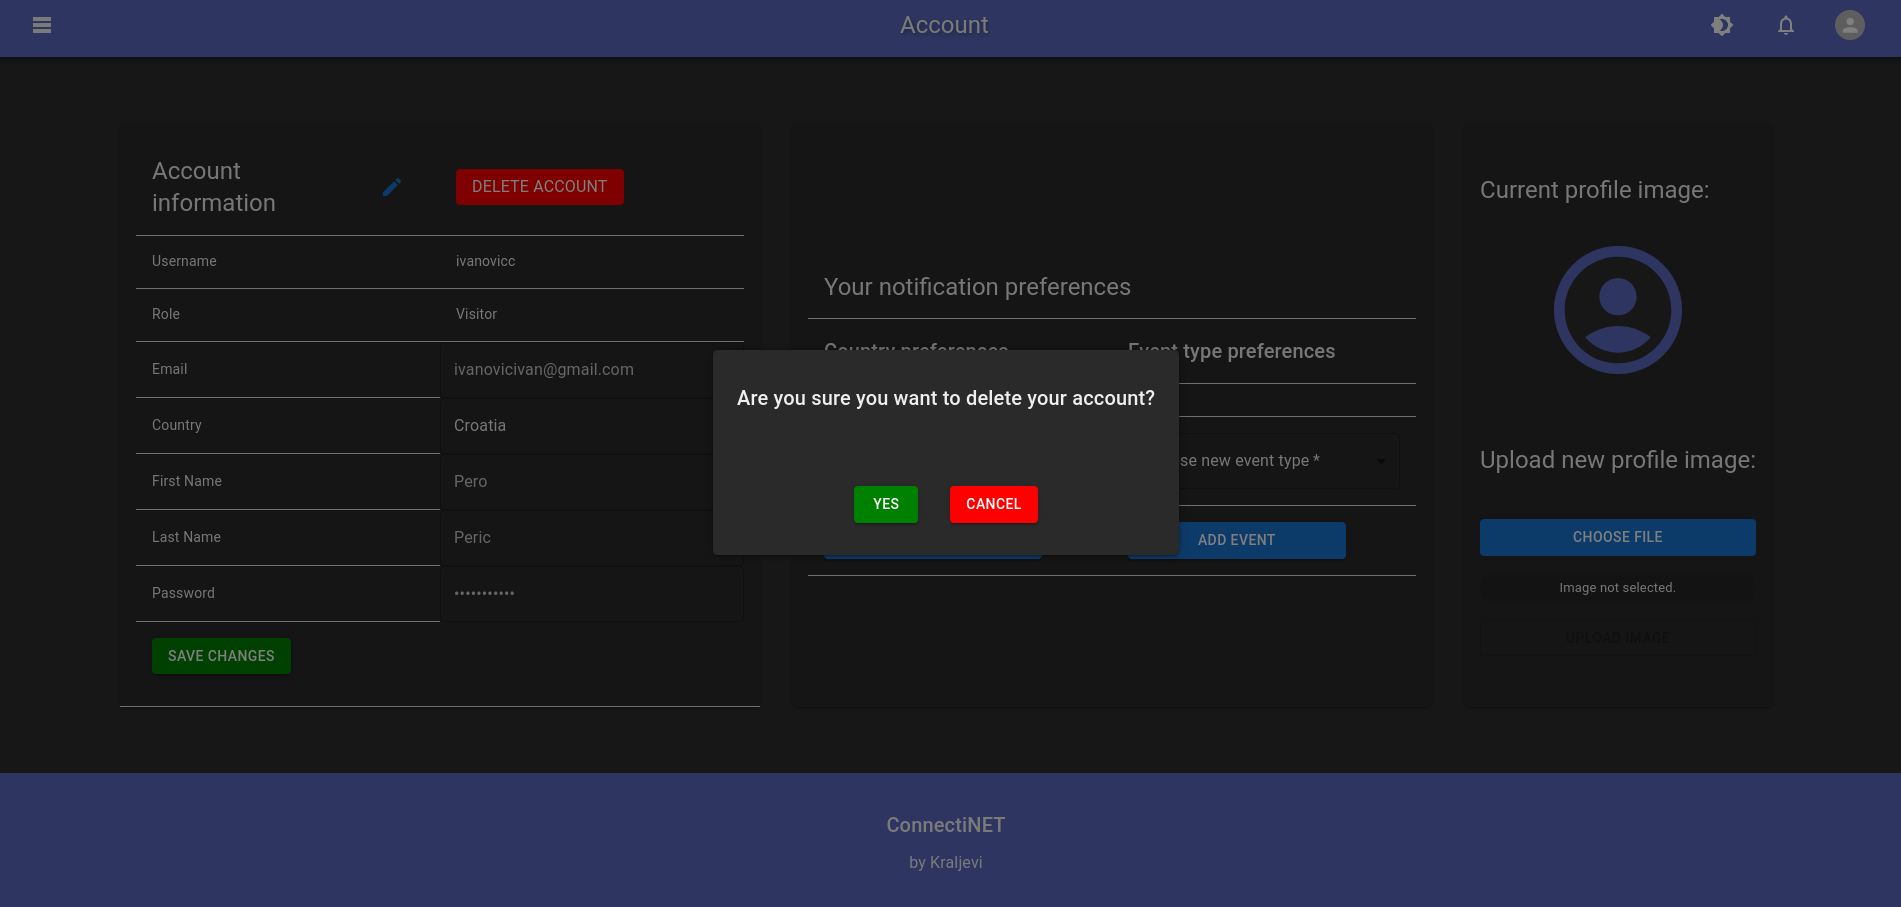
\includegraphics[width=1\textwidth]{slike/selenium_test_3.png}
					\caption{Testiranje brisanja korisničkog računa}
				\label{fig:my_image}
				\end{figure}

			\noindent \underbar{\textbf{Ispitni slučaj 4: Stvaranje novog događaja}}
			\begin{packed_item}

				\item  \textbf{Ulaz:}
				\item[] \begin{packed_enum}

					\item Otvaranje stranice za registraciju u web pregledniku
					\item Unos i odabir potrebnih podataka za kreiranje novog događaja
					\item Odabir opcije za "Create event"

				\end{packed_enum}
				
				\item  \textbf{Očekivani rezultat:}
				\item[] \begin{packed_item}
				\item[1] Uneseni podaci su vidljivi na stranici za kreiranje novog eventa
				\item[2.a] Događaj je uspješno kreiran
				\item[2.b] Neki od unesenih podataka je u neispravnom formatu, obavijest upozorava korisnika
				\end{packed_item}

				\item  \textbf{Rezultat:} Svi očekivani rezultati su ostvareni. Aplikacija je prošla test.
			\end{packed_item}


			\noindent \underbar{\textbf{Ispitni slučaj 5: Ostavljanje razine zainteresiranosti}}
			\begin{packed_item}

				\item  \textbf{Ulaz:}
				\item[] \begin{packed_enum}

					\item Otvaranje stranice za registraciju u web pregledniku
					\item Ulazak u detaljni prikaz o događaju klikom na "See more"
					\item Odabir razine zainteresiranosti

				\end{packed_enum}
				
				\item  \textbf{Očekivani rezultat:}
				\item[] \begin{packed_item}
				\item[1] Uneseni podaci su vidljivi na stranici za prijavu
				\item[2] Korisnik je oodabrao razinu zainteresiranosti
				\end{packed_item}

				\item  \textbf{Rezultat:} Svi očekivani rezultati su ostvareni. Aplikacija je prošla test.

			\end{packed_item}
			
			\eject 
		
		
		\section{Dijagram razmještaja}
			
			%\textbf{\textit{dio 2. revizije}}
			
			 %\textit{Potrebno je umetnuti \textbf{specifikacijski} dijagram razmještaja i opisati ga. Moguće je umjesto specifikacijskog dijagrama razmještaja umetnuti dijagram razmještaja instanci, pod uvjetom da taj dijagram bolje opisuje neki važniji dio sustava.}
			 Sustav je baziran na arhitekturi ”klijent – poslužitelj”, a klijenti koriste web preglednik kako bi pristupili web aplikaciji. Na poslužiteljskom računalu nalaze se poslužitelj frontend dijela web aplikacije, poslužitelj backend dijela web aplikacije te poslužitelj baze podataka. Backend dio aplikacije nalazi se unutar Docker kontejnera koji predstavlja okruženje koje sadrži sve što je potrebno za izvođenje dotičnog dijela aplikacije. Pohrana slika realizirana je uz pomoć usluge Firebase Storage koja je dio Firebase-a, platforme za razvoj mobilnih i web aplikacija. Firebase Storage se za pohranu i dohvat korisnički generiranih sadržaja oslanja na uslugu Google Cloud Storage. Sve spomenute usluge dio su šire platforme pod nazivom Google Cloud Platform (GCP). Odgovornost backend dijela web aplikacije je da prihvati generiranu javnu poveznicu na tu sliku i pohrani je u bazu podataka nakon što se korisnička slika otpremi na Firebase Storage. Firebase Storage omogućuje izravan prijenos datoteka od i do klijenta čime se rasterećuje poslužitelj koji samo procesuira poveznice. Komunikacija između osnovnih dijelova sustava odvija se preko HTTPS veze.
			 \begin{figure}[htbp]
				\centering
				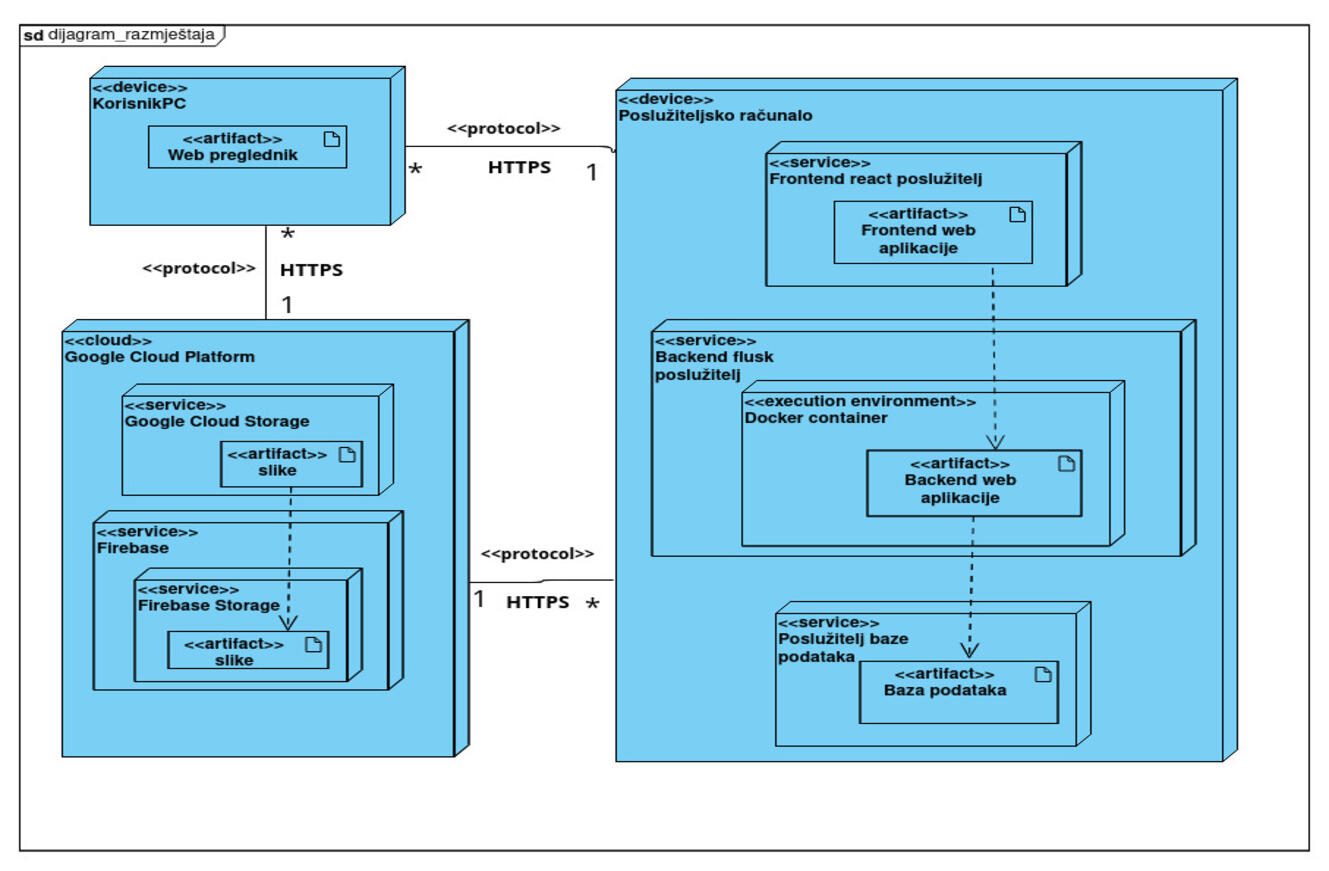
\includegraphics[width=1\textwidth]{dijagrami/diagram_razmjestaja_new2.jpeg}
				\caption{Dijagram razmještaja}
			\label{fig:my_image}
			\end{figure}
			\eject 

			
			\begin{document}
			
			\section{Upute za puštanje u pogon}
				
			\subsection{Priprema Lokalnog Razvojnog Okruženja}
			
			Za početak, potrebno je klonirati repozitorij s izvornim kodom na svoje računalo koristeći naredbu:
			\texttt{git clone \url{https://github.com/jetpans/ConnectiNET-kraljevi}} 
			Nakon toga je potrebno instalirati alate potrebne za pokretanje aplikacije lokalno:
			
			\begin{itemize}
					\item Instalirajte Docker i Docker Compose ili Docker Engine (\url{https://docs.docker.com/engine/install/})
					\item Instalirajte Node.js i npm za frontend (\url{https://nodejs.org/en/download})
					\item Instalirajte Python za backend (u slučaju da želite pokrenuti backend lokalno bez korištenja Docker kontejenera) (\url{https://www.python.org/downloads/})
					\item Instalirajte PostgreSQL bazu podataka (\url{https://www.postgresql.org/download/})
			\end{itemize}
			
			Za daljnji razvoj aplikacije preporuča se koristiti radno okruženje poput Visual Studio Code-a (\url{https://code.visualstudio.com/}). 
			
			\subsection{Postavljanje Backend-a s Docker Compose}
			
			U backend direktoriju se nalaze Dockerfile i docker-compose datoteke. Izvršite u naredbenom retku naredbu 
			\texttt{docker-compose up --build} 
			za izgradnju Docker kontejnera i pokretanje backend poslužitelja.
			
			\subsection{Konfiguracija PostgreSQL Baze Podataka}
			
			\subsubsection{Stvaranje PostgreSQL baze podataka}
			
			\begin{itemize}
					\item Prije nego što počnete, osigurajte da imate PostgreSQL instaliran na lokalnom sustavu.
					\item Koristite alat poput pgAdmin ili izravno putem terminala, stvorite novu bazu podataka za vašu aplikaciju.
					\item Definirajte korisnika i lozinku s odgovarajućim ovlastima na novoj bazi.
			\end{itemize}
			
			\subsubsection{Punjenje PostgreSQL Baze Podataka}
			
			Kako biste sagradili inicijalno stanje baze podataka, u razvojnoj fazi prvo smo napisali "SQLAlchemy" razrede koji modeliraju naše tablice u bazi podataka i spremili ih u datoteku models.py. Nakon toga, sagradili smo naše prazne entitete u bazi podataka sljedećim naredbama u python okruženju:
			
			\begin{verbatim}
			from models import app,db
			app.app_context().push()
			db.create_all()
			\end{verbatim}
			
			Osnovne podatke za vrstu događanja ručno smo unijeli u bazu koristeći "INSERT INTO" naredbe. Podatke za države kopirali smo iz javno dostupnog GitHub repozitorija te ih također unijeli koristeći "INSERT INTO" naredbe. Nakon unosa svih potrebnih inicijalnih vrijednosti u bazu, ovo stanje baze podataka spremili smo u datoteku backup.sql koristeći naredbu naredbenog retka:
			
			\begin{verbatim}
			pg_dump -c "<URI baze podataka>" > backup.sql
			\end{verbatim}
			
			Datoteka backup.sql sada ima sve potrebne PostgreSQL naredbe za čišćenje (-c) i unos starih podataka te se može koristiti za iniciranje baze podataka za vrijeme puštanja aplikacije u pogon.
			
			Bazu sada možemo puniti iz prije napravljene sigurnosne kopije sa svim potrebnim, unaprijed unesenim, podacima. To činimo naredbom naredbenog retka:
			
			\begin{verbatim}
			psql -d "<URI baze podataka>" -f backup.sql
			\end{verbatim}
			
			koja briše sve postojeće tablice i restaurira stanje baze podataka spremljeno u datoteci backup.sql.
			
			\subsection{Izgradnja i Pokretanje Frontend-a}
			
			Frontend direktorij sadrži izvorni kod React aplikacije. U njemu izvršite naredbu za instalaciju ovisnosti 

			\texttt{npm install}

			Za pokretanje razvojnog servera namijenjenog za lokalni razvoj aplikacije koristi se naredbama:
			
			\begin{verbatim}
			npm run start
			\end{verbatim}
			
			Za izgradnju optimiziranog produkcijskog koda izvršite naredbu:
			
			\begin{verbatim}
			npm run build
			\end{verbatim}
			
			Na kraju, za pokretanje Express servera koji poslužuje frontend koristi se naredba:
			
			\begin{verbatim}
			node app.js
			\end{verbatim}
			
			Nakon ovog koraka u potpunosti smo podigli lokalno razvojno okruženje i aplikacija je dostupna na \url{localhost:3000}. Za uspješan rad potrebno je i konfigurirati varijable okruženja, što je opisano u sljedećem koraku za puštanje u pogon na servis Render.
			
			\subsection{Puštanje u pogon na Render Platformu}
			
			Kreirajte račun na platformi Render (\url{https://render.com/}). Nakon što se ulogirate, redom dodajte:
			
			\begin{itemize}
					\item Novu PostgreSQL bazu podataka
					\item Novi web servis za backend dio aplikacije
					\begin{itemize}
							\item Preporučuje se koristiti github repozitorij s izvornim kodom, s tim da za root direktorij postavite vrijednost /backend.
							\item Za runtime odaberite Docker, a naredba za pokretanje je \texttt{gunicorn -w 4 -b 0.0.0.0:5000 run:app}.
							\item U varijable okruženja dodajte sve potrebne varijable:
							\begin{verbatim}
							FLASK_ENV (production za produkciju, development za razvoj)
							SECRET_KEY (vaš tajni ključ)
							DB_CONNECT_URL_PROD (Render url za povezivanje 
								s bazom podataka iz prethodnog koraka)
							MAIL_API_KEY (API ključ dobiven od Mailjet platforme)
							MAIL_SECRET (tajni ključ dobiven od Mailjet platforme)
							FIREBASE_URL (url dobiven od Firebase platforme)
							JWT_SECRET_KEY (tajni ključ za JWT token)
							\end{verbatim}
					\end{itemize}
					\item Novi web servis za frontend dio aplikacije
					\begin{itemize}
							\item Preporučuje se koristiti github repozitorij s izvornim kodom, s tim da za root direktorij postavite vrijednost /frontend.
							\item Za runtime odaberite Node.js, za build naredbu odaberite \texttt{npm install && npm run build}, a za start naredbu odaberite \texttt{node app.js}.
							\item U varijable okruženja dodajte sve potrebne varijable:
							\begin{verbatim}
							REACT_APP_API_URL (Render url za povezivanje 
								s backend poslužiteljem iz prethodnog koraka)
							HOST (0.0.0.0)
							PORT (3000)
							\end{verbatim}
					\end{itemize}
			\end{itemize}
			
			Render će automatski otkriti promjene u repozitoriju i pustiti u pogon aplikaciju u slučaju da ste odabrali opcije za automatsko puštanje u pogon pri kreaciji servisa. U suprotnom, možete ručno pokrenuti puštanje u pogon. Aplikacija je sada dostupna na url-u dobivenom od Render platforme. Odlaskom na dobiveni url vidjet ćemo ekran za prijavu aplikacije ConnectiNET. Moguće je i direktno pristupiti backend poslužitelju na url-u dobivenom od Render platforme.
			\eject 
	\chapter{Zaključak i budući rad}
		
		\textbf{\textit{dio 2. revizije}}\\
		
		 \textit{U ovom poglavlju potrebno je napisati osvrt na vrijeme izrade projektnog zadatka, koji su tehnički izazovi prepoznati, jesu li riješeni ili kako bi mogli biti riješeni, koja su znanja stečena pri izradi projekta, koja bi znanja bila posebno potrebna za brže i kvalitetnije ostvarenje projekta i koje bi bile perspektive za nastavak rada u projektnoj grupi.}
		
		 \textit{Potrebno je točno popisati funkcionalnosti koje nisu implementirane u ostvarenoj aplikaciji.}
		
		\eject 
	\chapter*{Popis literature}
		\addcontentsline{toc}{chapter}{Popis literature}
	 	
 		\textbf{\textit{Kontinuirano osvježavanje}}
	
		\textit{Popisati sve reference i literaturu koja je pomogla pri ostvarivanju projekta.}
		
		
		\begin{enumerate}
			
			
			\item  Programsko inženjerstvo, FER ZEMRIS, \url{http://www.fer.hr/predmet/proinz}
			
			\item  I. Sommerville, "Software engineering", 8th ed, Addison Wesley, 2007.
			
			\item  T.C.Lethbridge, R.Langaniere, "Object-Oriented Software Engineering", 2nd ed. McGraw-Hill, 2005.
			
			\item  I. Marsic, Software engineering book``, Department of Electrical and Computer Engineering, Rutgers University, \url{http://www.ece.rutgers.edu/~marsic/books/SE}
			
			\item  The Unified Modeling Language, \url{https://www.uml-diagrams.org/}
			
			\item  Astah Community, \url{http://astah.net/editions/uml-new}
		\end{enumerate}
		
		 
	
	
	\begingroup
	\renewcommand*\listfigurename{Indeks slika i dijagrama}
	%\renewcommand*\listtablename{Indeks tablica}
	%\let\clearpage\relax
	\listoffigures
	%\vspace{10mm}
	%\listoftables
	\endgroup
	\addcontentsline{toc}{chapter}{Indeks slika i dijagrama}


	
	\eject 
		
	\chapter*{Dodatak: Prikaz aktivnosti grupe}
		\addcontentsline{toc}{chapter}{Dodatak: Prikaz aktivnosti grupe}
		
		\section*{Dnevnik sastajanja}
		
		%&\textbf{\textit{Kontinuirano osvježavanje}}\\
		%\textit{U ovom dijelu potrebno je redovito osvježavati dnevnik sastajanja prema predlošku.}
		
		\begin{packed_enum}
			\item  sastanak
			\item[] \begin{packed_item}
				\item Datum: 19. listopada 2023.
				\item Prisustvovali: L. Miličević, M. Papak, F. Aleksić, S. Đelekovčan, D. Sviličić, E. Pužar
				\item Teme sastanka:
				\begin{packed_item}
					\item  sastanak s asistenticom i demonstratorom
					\item  uvod u temu projekta
				\end{packed_item}
			\end{packed_item}

			\item  sastanak
			\item[] \begin{packed_item}
				\item Datum: 22. listopada 2023.
				\item Prisustvovali: L. Miličević, M. Papak, F. Aleksić, D. Huljev, S. Đelekovčan, D. Sviličić, E. Pužar
				\item Teme sastanka:
				\begin{packed_item}
					\item  analiza teme projekta
					\item  korištenje git-a i github-a
					\item  konačan odabir alata i tehnologija
					\item  uvod u naš github repozitorij
				\end{packed_item}
			\end{packed_item}
			
			\item  sastanak
			\item[] \begin{packed_item}
				\item Datum: 30. listopada 2023.
				\item Prisustvovali: L. Miličević, D. Huljev, S. Đelekovčan, D. Sviličić, E. Pužar
				\item Teme sastanka:
				\begin{packed_item}
					\item  definiranje funkcionalnih zahtjeva
					\item  podjela opisa obrazaca uporabe, opisa zadatka i arhitekture sustava
				\end{packed_item}
			\end{packed_item}

			\item  sastanak
			\item[] \begin{packed_item}
				\item Datum: 2. studenoga 2023.
				\item Prisustvovali: L. Miličević, M. Papak, F. Aleksić, D. Huljev, S. Đelekovčan, D. Sviličić, E. Pužar
				\item Teme sastanka:
				\begin{packed_item}
					\item  analiza do sada napravljenih funkcionalih zahtjeva
					\item  diskusija o modeliranju baze podataka
				\end{packed_item}
			\end{packed_item}
			
			%
			
		\end{packed_enum}
		
		\eject
		\section*{Tablica aktivnosti}
		
			%\textbf{\textit{Kontinuirano osvježavanje}}\\
			
			%\textit{Napomena: Doprinose u aktivnostima treba navesti u satima po članovima grupe po aktivnosti.}

			\begin{longtblr}[
					label=none,
				]{
					vlines,hlines,
					width = \textwidth,
					colspec={X[7, l]X[1, c]X[1, c]X[1, c]X[1, c]X[1, c]X[1, c]X[1, c]}, 
					vline{1} = {1}{text=\clap{}},
					hline{1} = {1}{text=\clap{}},
					rowhead = 1,
				} 
			
				\SetCell[c=1]{c}{} & \SetCell[c=1]{c}{\rotatebox{90}{\textbf{Luka Miličević}}} & \SetCell[c=1]{c}{\rotatebox{90}{\textbf{Duje Huljev}}} &	\SetCell[c=1]{c}{\rotatebox{90}{\textbf{Filip Aleksić}}} & \SetCell[c=1]{c}{\rotatebox{90}{\textbf{Mate Papak}}} &	\SetCell[c=1]{c}{\rotatebox{90}{\textbf{Stjepan Đelekovčan}}} & \SetCell[c=1]{c}{\rotatebox{90}{\textbf{Domagoj Sviličić}}} &	\SetCell[c=1]{c}{\rotatebox{90}{\textbf{Erik Pužar}}} \\  
				Upravljanje projektom 		& 3 &  &  &  &  &  & \\ 
				Opis projektnog zadatka 	& 3 &  &  &  &  &  & \\ 
				
				Funkcionalni zahtjevi       &  &  &  &  &  &  &  \\ 
				Opis pojedinih obrazaca 	&  &  &  &  &  &  &  \\ 
				Dijagram obrazaca 			&  &  &  &  &  &  &  \\ 
				Sekvencijski dijagrami 		&  &  &  &  &  &  &  \\ 
				Opis ostalih zahtjeva 		& 0.5 &  &  &  &  &  &  \\ 

				Arhitektura i dizajn sustava	 & 2 &  &  &  &  &  &  \\ 
				Baza podataka				&  &  &  &  &  &  &   \\ 
				Dijagram razreda 			&  &  &  &  &  &  &   \\ 
				Dijagram stanja				&  &  &  &  &  &  &  \\ 
				Dijagram aktivnosti 		&  &  &  &  &  &  &  \\ 
				Dijagram komponenti			&  &  &  &  &  &  &  \\ 
				Korištene tehnologije i alati 		&  &  &  &  &  &  &  \\ 
				Ispitivanje programskog rješenja 	&  &  &  &  &  &  &  \\ 
				Dijagram razmještaja			&  &  &  &  &  &  &  \\ 
				Upute za puštanje u pogon 		&  &  &  &  &  &  &  \\  
				Dnevnik sastajanja 			&  &  &  &  &  &  &  \\ 
				Zaključak i budući rad 		&  &  &  &  &  &  &  \\  
				Popis literature 			&  &  &  &  &  &  &  \\  
				&  &  &  &  &  &  &  \\ \hline 
				\textit{Dodatne stavke kako ste podijelili izradu aplikacije} 			&  &  &  &  &  &  &  \\ 
				\textit{npr. izrada početne stranice} 				&  &  &  &  &  &  &  \\  
				\textit{izrada baze podataka} 		 			&  &  &  &  &  &  & \\  
				\textit{spajanje s bazom podataka} 							&  &  &  &  &  &  &  \\ 
				\textit{back end} 							&  &  &  &  &  &  &  \\  
				 							&  &  &  &  &  &  &\\ 
			\end{longtblr}
					
					
		\eject
		\section*{Dijagrami pregleda promjena}
		
		\textbf{\textit{dio 2. revizije}}\\
		
		\textit{Prenijeti dijagram pregleda promjena nad datotekama projekta. Potrebno je na kraju projekta generirane grafove s gitlaba prenijeti u ovo poglavlje dokumentacije. Dijagrami za vlastiti projekt se mogu preuzeti s gitlab.com stranice, u izborniku Repository, pritiskom na stavku Contributors.}
		
	


\end{document} %naredbe i tekst nakon ove naredbe ne ulaze u izgrađen dokument 


